\documentclass[dsc,numbers]{coppe}
% qualificacao - dscexam
% tese - dsc

\usepackage{amsmath,amssymb, amsthm}
\usepackage{hyperref}
\usepackage[utf8]{inputenc}
\usepackage{graphicx}
\usepackage[caption=false]{subfig}
%\usepackage{ifthen}
\usepackage{color}
\usepackage{array}
\usepackage{colortbl}
\usepackage[algoruled,lined,boxed]{algorithm2e}
\usepackage{lineno,setspace}
\usepackage{eqparbox}
\usepackage{indentfirst}
\usepackage{braket}
\usepackage{amsfonts}
\usepackage{fancyhdr}
\usepackage{comment}
\usepackage{float}
\usepackage{pdfpages}
\usepackage{enumitem}
\usepackage{lscape}
\usepackage[export]{adjustbox}
%\usepackage{cite}
%\usepackage{subfigure}

%\usepackage{caption}    
%\usepackage{subcaption} 

\usepackage{makeidx} % sugestão... caso você queira fazer um índice

\newtheorem{theorem}{Teorema}[chapter]
\newtheorem{example}[theorem]{Exemplo}
\newtheorem{conjecture}[theorem]{Conjectura}
\newtheorem{observation}[theorem]{Observa\c{c}\~ao}
\newtheorem{lemma}[theorem]{Lema}
\newtheorem{proposition}[theorem]{Proposi\c{c}\~ao}
\newtheorem{fac}[theorem]{Fato}
\newtheorem{corollary}[theorem]{Corol\'ario}
\newtheorem{lema}[theorem]{Lema}
\newtheorem{definition}[theorem]{Defini\c{c}\~ao}
%\newenvironment{proof}[1][Demonstra\c{c}\~ao]{\emph{#1.} }{\ \hfill$\square$}

\newenvironment{proofidea}{\par\noindent\textit{Justificativa.}}{\hfill$\square$}


\newcommand\floor[1]{\left\lfloor #1 \right\rfloor}
\newcommand\toricclass[1]{#1_\circ^\circ}
\newcommand{\toric}[1]{\left[#1\right]^\circ_\circ}
\renewcommand\mod[1]{\!\!\!\!\!\pmod{#1}}

%\usepackage{xparse}% http://ctan.org/pkg/xparse
%\NewDocumentCommand{\ceil}{s O{} m}{%
%  \IfBooleanTF{#1} % starred
%    {\left\lceil#3\right\rceil} % \ceil*[..]{..}
%    {#2\lceil#3#2\rceil} % \ceil[..]{..}
%}%Para função matematica piso/teto

\makelosymbols
\makeloabbreviations

\makeindex  % Se não tiver indice remissivo pode remover

\begin{document}
\title{Estudo de Grafos de Intersecção de Caminhos}
  \foreigntitle{Some Remarks About Intersection Graphs of Paths on Grid}
  \author{Tanilson Dias dos}{Santos}
  \advisor{Prof.}{Jayme Luiz}{Szwarcfiter}{Ph.D.}  
  \advisor{Prof.}{Uéverton dos Santos}{Souza}{D.Sc.}
\advisor{Prof.}{Claudson Ferreira}{Bornstein}{Ph.D.}

 \examiner{Prof.}{Jayme Luiz Szwarcfiter}{Ph.D.}
    \examiner{Prof.}{Uéverton dos Santos Souza}{D.Sc.}
 \examiner{Prof.}{Claudson Ferreira Bornstein}{Ph.D.}
 \examiner{Prof.}{Liliana Alcón}{D.Sc.}
 \examiner{Prof.}{María Pía Mazzoleni}{D.Sc.}
 \examiner{Prof.}{Márcia Rosana Cerioli}{D.Sc.}
  
  %\examiner{Prof.}{Nome do Quinto Examinador Sobrenome}{Ph.D.}
  \department{PESC}
  \date{09}{2020}

  \keyword{Edge Path}
  \keyword{Grid Path}
  \keyword{Intersections}
  \keyword{search}

  \maketitle

  \frontmatter
  \dedication{Dedico à minha filha, Ana Flor de Lis, e à minha esposa, Juliana Pontes.
  Dedico também aos meus avós maternos, Teobaldo Ferreira Dias (\textit{in memoriam}) e Lídia Andrade Ferreira (\textit{in memoriam}), e paternos,
  Armando Bento de Oliveira e Josefa Ericino de Oliveira (\textit{in memoriam}).
  }

  \chapter*{Agradecimentos}

Quando pensei em fazer o doutorado não fazia ideia do quanto minha vida se transformaria. A boa notícia é que mudou para melhor!

Não poderia deixar de fazer alguns agradecimentos aos envolvidos direta ou indiretamente na minha pesquisa e que possibilitaram trilhar essa jornada. 

Agradeço a Deus, pela sua misericórdia e providência em minha vida.

Agradeço do fundo do meu coração e com todas as forças à minha mãe, Tânia Andrade, que me educou, me ensinou a ler e escrever, sempre orou por mim, lutou para que eu sempre tivesse uma boa educação, me ajudou financeiramente quando eu precisei e sempre me incentivou a estudar e dar o melhor de mim. Apesar de uma origem humilde essa mulher pelejou para que eu pudesse concretizar o sonho do doutorado. Obrigado mãe.

À minha irmã por estar presente na minha vida e pelo incentivo não apenas na minha vida acadêmica, mas principalmente no âmbito pessoal.

Agradeço aos meus amigos e familiares, principalmente à minha esposa, Juliana, pela compreensão com minha falta de atenção e pela minha ausência durante este período.

Aos professores que tive na cidade de Brejinho de Nazaré que contribuíram para minha formação básica; aos professores que tive em Palmas, durante a graduação, que foram responsáveis pela minha formação superior; e finalmente aos professores que tive no mestrado e no doutorado por todo o conhecimento compartilhado no período de pós-graduação.

Aos inúmeros amigos que fiz no LAC, Laboratório de Algoritmos e Combinatória, e no PPGI, Programa de Pós-graduação em Informática, com os quais pude aprender muito e comungar de momentos de estudo e descontração.

Aos meus orientadores, Jayme, Claudson e Uéverton, por serem luz, sobriedade, ajuda, professores e amigos ao longo do tempo em que trabalhamos juntos.

Aos demais membros da banca, professoras Márcia Cerioli, Maria Pía e Liliana Alcón por avaliarem e contribuírem com este trabalho.

Não poderia deixar de reconhecer com gratidão o estágio doutoral feito na Universidade Nacional de La Plata - UNLP, Argentina. Agradeço à acolhida que tive na Argentina e na UNLP personificados nas pessoas das professoras Maria Pía e Liliana Alcón.


Agradeço ao colegiado do curso de Ciência da Computação, e demais instâncias da Universidade Federal do Tocantins que colaboraram para meu afastamento para qualificação doutoral.



Também merece um agradecimento  a rede de cafés Starbucks onde muitas vezes me retirei para escrever alguns artigos. 


À Coordenação de Aperfeiçoamento 
de Pessoal de Nível Superior - Brasil (CAPES) pelo financiamento parcial dessa pesquisa.

  \begin{abstract}
Golumbic, Lipshteyn e Stern definiram em 2009 a classe de grafos EPG, uma classe de grafos de intersecção baseada na intersecção de arestas em caminhos sobre uma grade. Um grafo EPG $G$ é um grafo que admite uma representação onde seus vértices correspondem a caminhos em uma grade $Q$, tal que dois vértices de $G$ são adjacentes se e somente se os caminhos correspondentes em $Q$ tem pelo menos uma aresta comum. Se os caminhos na representação tem no máximo $k$ mudanças de direção (dobras), dizemos que  essa é uma representação $B_k$-EPG. Uma coleção $C$ de conjuntos satisfaz a propriedade Helly quando toda subcoleção de $C$ que é mutuamente intersectante possui no mínimo um elemento comum. Neste trabalho mostramos que  o problema de reconhecimento de grafos  $B_k$-EPG-Helly %, de um grafo   $G=(V,E)$, cujas aresta-intersecções de caminhos em uma grade satisfaz a propriedade Helly, então chamados grafos  $B_k$-EPG-Helly, 
 está em  $\mathcal{NP}$, para todo $k$ limitado por uma função polinomial de $|V(G)|$. Além disto, mostramos que o reconhecimento de grafos $B_1$-EPG-Helly é $NP$-completo, e ele permanece   $NP$-completo mesmo quando restrito aos grafos   2-apex e 3-degenerado.


Palavras-chave: Aresta-intersecção de caminhos sobre uma grade, Propriedade Helly, Grafos de Intersecção, $NP$-completude, Dobra simples.
\end{abstract}

  \begin{foreignabstract}
Golumbic, Lipshteyn and Stern defined in 2009 the class of EPG graphs, an intersection graph class  based on edge intersection of paths on a grid. An EPG graph $G$ is a graph that admits a representation where its vertices correspond to paths in a grid $Q$, such that two vertices of $G$ are adjacent if and only if the corresponding paths in $Q$ have a common edge. If the paths in the representation have at most $k$ changes of direction  (bends), we say that this is a  $B_k$-EPG representation. A collection $C$ of sets satisfies the Helly property when every sub-collection of $C$ that is pairwise intersecting has at least a common element. In this paper we show that the problem of  recognizing $B_k$-EPG-Helly graphs  
% $G=(V,E)$ whose edge-intersections of paths in a grid satisfy the Helly property, so-called $B_k$-EPG-Helly graphs, 
 is in $\mathcal{NP}$, for every $k$ bounded by a polynomial function of $|V(G)|$. In addition, we show that recognizing $B_1$-EPG-Helly graphs is $NP$-complete, and it remains $NP$-complete even when restricted to 2-apex and 3-degenerate graphs.



Keywords: Edge-intersection of paths on a grid, Helly property, Intersection graphs, $NP$-completeness, Single bend paths.

\end{foreignabstract}



  \tableofcontents
  \listoffigures
  %\listoftables
  \printlosymbols
  \printloabbreviations

  \mainmatter
  \chapter{Introdução}

\begin{flushright}
\begin{minipage}[t][0cm][b]{0.47\textwidth}
\emph{Se não podes entender, crê para que entendas. A fé precede, o intelecto segue.}
\end{minipage}

\rule[0cm]{7cm}{0.03cm}%{largura}{espessura}

Santo Agostinho
\end{flushright}


\section{Motivação e objetivos}

Um grafo EPG $G$ é um grafo que admite uma representação em que seus vértices são representados por caminhos de uma grade $Q$, tal que dois vértices de $G$ são adjacentes se e somente se os caminhos correspondestes tem no mínimo uma aresta em comum.

% The searches on path intersection graph are approached considering intersections from vertices or edges. Cases where models of intersection have a tree as host appear first in the literature e.g. \cite{gavril1974intersection, golumbic1985edge, golumbic1985}, later representations on a grid were considered, e.g. \cite{golumbic2009,golumbic2013, golumbic2013intersection}. More details on each intersection model will be given in the following text.

% The research of paths whose host is a tree starts in 1974 with Gavril~\cite{gavril1974intersection} who proved that a graph $G$ is an intersection graph of subtrees family of a tree if and only if $G$ is a chordal graph. An undirected graph $G$ is called an EPT graph if it is the edge intersection graph of a family of paths in a tree. Let $P$ be a family of paths on a host tree $T$ . Two types of intersection graphs from the pair $<P,T>$ are defined, namely VPT and EPT graphs.
% The \textit{edge intersection graph} of $P$, EPT(P), has vertices which correspond to the members of P, and two vertices are adjacent in EPT(P) if and only if the corresponding paths in P share at least one edge in T. Similarly, the \textit{vertex intersection graph} of P, VPT(P), has vertices which correspond to the members of P, and two vertices are adjacent in VPT(P) if and only if the corresponding paths in P share at least one vertex in T.

% VPT and EPT graphs are incomparable families of graphs. However, when the maximum degree of the host tree is restricted to 3 the family of
% VPT graphs coincides with the family of EPT graphs, \cite{alcon2010necessary}.

%  Golumbic, Lipshteyn and Stern defined in 2009 the class of EPG graphs, as the  intersection graph of edge paths on a grid. An EPG graph $G$ is a graph that admits a representation where its vertices correspond to paths in a grid $Q$, such that two vertices of $G$, we say $v_1$ and $v_2$, they are adjacent if and only if their corresponding paths $P_{v_1}$ and $P_{v_2}$, they have a common edge in $Q$. If the paths in the representation have at most $k$ changes of direction  (bends), we say that it is a  $B_k$-EPG representation. In particular when the paths of this representation have at most 1 bend we say that this is a $B_1$-EPG representation or single bend representation for EPG graphs.  A collection $C$ of sets satisfies the Helly property when every sub-collection of $C$ that is pairwise intersecting has at least one common element. 




O estudo de grafos EPG tem motivação relacionada com o problema de \textit{design} VLSI que combina a noção de grafos de intersecção de arestas de caminhos em uma árvore com um modelo de \textit{layout} de grade VLSI~\cite{golumbic2009}. O número de dobras em um circuito integrado pode aumentar a área de \textit{layout} e consequentemente aumentar o custo de produção do microchip. 
Essa é uma das principais aplicações que instigam a  pesquisa sobre representações EPG de algumas famílias de grafos quando existem restrições no número de dobras nos caminhos usados na representação.
Outras aplicações e detalhes sobre problemas de \textit{layout} de circuitos podem ser encontrados em~\cite{bandy1990, molitor1991}.   

Um grafo é $ B_k$-EPG se ele admite uma representação (sobre uma grade) em que cada caminho possua no máximo $k$ dobras. A título de exemplo a Figura~\ref{fig:trianguloepgRepresentacao}(a) retrata um grafo $C_3$, a Figura~\ref{fig:trianguloepgRepresentacao}(b) retrata uma representação EPG do grafo $C_3$ onde os caminhos não possuem dobra e a  Figura~\ref{fig:trianguloepgRepresentacao}(c) retrata uma representação com 1 dobra do grafo $C_3$. Consequentemente, $C_3$ é um grafo  $B_0$-EPG. %De forma mais geral, grafos $B_0$-EPG coincidem com grafos de intervalo~\cite{golumbic2009}.

O \emph{número de dobras} de uma classe de grafos é o menor  $k$ para o qual todos os grafos na classe possuem uma representação $B_k$-EPG. Grafos de intervalo possuem número de dobras $0$~\cite{golumbic2009}, árvores possuem  número de dobras $1$~\cite{golumbic2009} e  grafos outerplanar possuem número de dobras $2$~\cite{daniel2014b}. O número de dobras da classe dos grafos planares é um problema em aberto, porém sabe-se que ele é $ 3 $ ou $4$~\cite{daniel2014b}. %Apesar de existirem demonstrações de que o número de dobras não é maior que 4 para a classe dos grafos planares, também não se conhece algum grafo planar que não possa ser representado com 3 dobras.

A classe dos grafos EPG tem sido estudada em diversos trabalhos, tais como  \cite{alcon2016, Asinowski2009, cohen2014, golumbic2009, heldt2014,  martin2017}, entre outros. As investigações frequentemente abordam caracterizações com relação número de dobras das representações de um grafo. A respeito da complexidade de reconhecimento de grafos $B_k$-EPG, somente a complexidade de reconhecimento de três subclasses de grafos EPG foi determinada:
 grafos $B_0$-EPG podem ser reconhecidos em tempo polinomial, uma vez que correspondem a classe de grafos de intervalo, ver~\cite{booth1976, golumbic2009}. Em contraste, o reconhecimento das classes $B_1$-EPG e $B_2$-EPG é $NP$-completo, ver~\cite{heldt2014, martin2017}.

\begin{figure}[h]
  \centering
  \begin{tabular}{ c p{0.15cm} c p{0.15cm} c }
    %\centering
    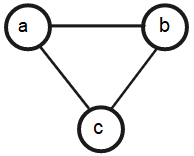
\includegraphics[width=2.3cm]{./img/trianguloabc.png} && 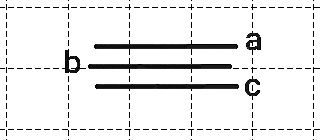
\includegraphics[width=3.5cm]{./img/b0epgTransparenciaGrade2.png} & &
    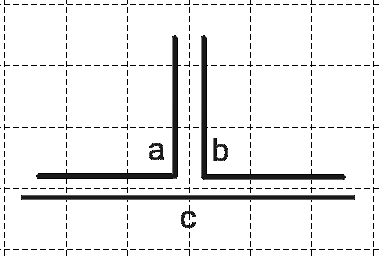
\includegraphics[width=3.5cm]{./img/b1EpgTransparenteGrade2.png}
    \\
    \footnotesize %\centering 
    (a) O grafo $C_3$ && \footnotesize(b) Representação $B_0$-EPG de $C_3$ && \footnotesize (c) Representação $B_1$-EPG de $C_3$\\

  \end{tabular}

 \caption{O grafo $ C_3 $ com duas representações, uma sem dobra e outra com uma dobra} \label{fig:trianguloepgRepresentacao}
\end{figure}


%A  collection $C$ of sets satisfies the Helly property when every sub-collection of $ C $ that is pairwise intersecting has at least one common element. The Helly property has this name in honor of the great Austrian mathematician Eduard Helly, who in 1923 proposed his famous theorem concerning the relation of intersecting sets.

%The study of the Helly property is useful in very diverse areas of science, and we can enumerate applications in semantics, code theory, computational biology, database, image processing, graph theory, optimization, and linear programming \cite{dourado2009}.

%Note that the representation of Figure~\ref{fig:trianguloepgRepresentacao}(b) satisfies the Helly property, while the representations of Figures~\ref{fig:trianguloepgRepresentacao}(c) and~\ref{fig:trianguloepgRepresentacao}(d) do not satisfy it.

Este trabalho propõe o estudo de grafos que possuem uma representação EPG-Helly. 
A propriedade Helly relacionada com representações EPG foi  estudada em~\cite{golumbic2009} e \cite{golumbic2013}. Em particular, esses trabalhos determinaram um parâmetro conhecido como número de Helly forte  para grafos $B_1$-EPG. 

Estão no escopo de interesse deste trabalho os seguintes tópicos:

\begin{itemize}
    
    \item Determinar a complexidade de reconhecimento de grafos $B_1$-EPG-Helly;
    \item Determinar limites superiores e/ou inferiores para os parâmetros número de Helly e número de Helly forte em grafos EPG e EPG-Helly;
    
    \item Estudar os parâmetros número de Helly e número de Helly forte também em grafos de intersecção de vértices em caminhos sobre grade (VPG e VPG-Helly);
    
    \item Encontrar classes de grafos para os quais os resultados possam se estender.
\end{itemize}



% \section{Motivação}
% Por que pesquisar?

% Qual a relevância do problema e por que escolher esse tema?

% Qual é o problema estudado?
% Onde ele acontece?
% Quem observou ou observa sua ocorrência?
% Por que isso é importante e deve ser solucionado?

% \section{Objetivo}

% Quais as finalidades intelectuais?

% verificar... compreender... analizar...
% comparar...

\section{Organização do texto}

No Capítulo 2 apresentaremos algumas definições básicas sobre grafos juntamente com uma breve explicação sobre a propriedade Helly. Além disso, o capítulo aborda uma breve discussão sobre problemas de caminhos em grade.

O Capítulo 3 será dedicado à definição do problema estudado, análise de algumas representações EPG básicas e demonstração da $NP$-completude do problema de reconhecimento de grafos $B_1$-EPG-Helly. São publicações resultantes desta pesquisa, os seguintes escritos:

\begin{enumerate}
    \item BORNSTEIN, C. F.; SANTOS, T. D.; SOUZA, U. S.; SZWARCFITER, J. L. A Complexidade do Reconhecimento de Grafos B1-EPG-Helly. In: 50º SBPO - Simpósio Brasileiro de Pesquisa Operacional, 2018, Rio de Janeiro. Cidades Inteligentes: Planejamento Urbano, Fontes Renováveis e Distribuição de Recursos, 2018.

     \item BORNSTEIN, C. F.; SANTOS, T. D.; SOUZA, U. S.; SZWARCFITER, J. L. Sobre a Dificuldade de Reconhecimento de Grafos B1-EPG-Helly. In: XXXVIII Congresso da Sociedade Brasileira de Computação, 2018, Natal - RN. Computação e Sustentabilidade, 2018. p. 113-116.

     
     \item BORNSTEIN, C. F.; SANTOS, T. D.; SOUZA, U. S.; SZWARCFITER, J. L. The complexity of B1-EPG-Helly graph recognition. In: VIII Latin American Workshop On Cliques in Graphs (LAWCG), ICM 2018 Satellite Event, 2018, Rio de Janeiro. Program and Abstracts, 2018. p. 69.

     
     \item BORNSTEIN, C. F.; GOLUMBIC, M.C.; SANTOS, T. D.; SOUZA, U. S.; SZWARCFITER, J. L.  The complexity of B1-EPG-Helly graph recognition. %In:  45th International Workshop on Graph-Theoretic Concepts in Computer Science,  2019, Vall de Núria, Catalonia, Spain. 
     (Submited).
     
\end{enumerate}


Por fim, no Capítulo 4, discutimos os principais resultados obtidos para grafos EPG. Adicionalmente, teremos
também as considerações finais sobre o trabalho aqui apresentado com algumas perspectivas e ideias sobre o problema e possíveis direcionamentos para novos estudos de trabalhos futuros.
  \chapter{Grafos de interseção de caminhos em grades e em árvores}\label{Notions}


\begin{flushright}
\begin{minipage}[t][0cm][b]{0.47\textwidth}
\emph{Se você conhece o inimigo e conhece a si mesmo, não precisa temer o resultado de cem batalhas. }
\end{minipage}

\rule[0cm]{7cm}{0.03cm}%{largura}{espessura}

Sun Tzu
\end{flushright}

\section{Conceitos e definições iniciais}

Neste capítulo apresentaremos alguns conceitos que facilitarão o entendimento do problema estudado. Em geral, a maioria das notações utilizadas é simples, então vamos procurar ilustrar com exemplos somente aqueles conceitos e definições que fogem ao escopo básico da teoria de grafos. Como bibliografia básica sobre grafos sugerimos a leitura de~\cite{jayme2018}.

É importante ressaltar que em todo esse estudo, somente consideraremos grafos finitos, conexos e simples, ou seja, grafos sem
laços (aresta ligando um vértice nele mesmo) ou mais de uma aresta ligando dois
vértices.

A seguir descreve-se a terminologia e notação utilizada neste trabalho.

Um grafo $G$ é uma estrutura composta por dois subconjuntos finitos: $V(G)$ é o subconjunto cujos elementos são denominados \emph{vértices}, e $E(G)$ é subconjunto de pares não ordenados de elementos tomados de $V(G)$, os quais são chamados de \emph{arestas}. Uma aresta $e = (u,v)\in E(G)$ é formada pelo par de vértices $u,v \in V(G)$, neste caso $u$ e $v$ são ditos ser vértices \emph{adjacentes}. Dizemos também que  $e$ é \emph{aresta incidente} a $u$ e $v$. Denotamos a \emph{cardinalidade} de $|V(G)| = n$ e $|E(G)| = m$.

A \emph{vizinhança aberta} de um vértice $v\in V(G)$ é denotada $N(v) = \{u\in V(G) | (u,v) \in E(G)\}$. Já a \emph{vizinhança fechada} de um vértice $v\in V(G)$ é denotada $N[v] = N(v) \cup \{v\}$. 

Sejam $u, v$ vértices de $G$, se $N(u) = N(v)$ então $u$ e $v$ são ditos \emph{gêmeos falsos}, por outro lado, se $N[u] = N[v]$, então $u$ e $v$ são ditos \emph{gêmeos verdadeiros}. O \emph{grau de um vértice} $v$, denotado por $d(v)$, corresponde ao número de vértices adjacentes a $v$, ou seja, a cardinalidade de $|N(v)|$. O \emph{grau máximo} de um grafo $G$ é denotado por $\Delta(G) = max\{d(v) | v \in V(G)\}$. De forma similar o \emph{grau mínimo} é denotado por $\delta(G) = min\{d(v) | v \in V(G)\}$.

Dado um grafo $G$, e um vértice $v \in V(G)$, o grafo $G\backslash \{v\}$ é obtido a partir de $G$ retirando-se o vértice $v$ de seu conjunto de vértices, e retirando-se também todas arestas de $E(G)$ incidentes a $v$. De forma semelhante, dada uma aresta $e \in E(G)$, o grafo $G\backslash \{e\}$ é obtido a partir de $G$ retirando-se a aresta $e$ de $E(G)$.

Dizemos que $G'(V',E')$ é um \emph{subgrafo} de um grafo $G(V,E)$ quando $V'\subseteq V$ e $E'\subseteq E$. Quando o subgrafo $G'$ contém todas as arestas de $E$ cujas extremidades estão contidas em $V'$, então $G'$ é o \emph{subgrafo induzido} de $G$ por $V'$.  

Um grafo $G$ é um \emph{ciclo}, que denotaremos por $C_n$, se ele é uma sequência de vértices   $v_1, \dots, v_n, v_1$ distintos, onde $v_i \neq v_j$ para $i\neq j$ e $(v_i, v_{i+1})\in E(G)$,  tal que $n\geq 3$. 

Um grafo que não possui ciclos é dito \emph{acíclico}. Um grafo $G$ é \emph{conexo} se existe um caminho entre qualquer par de vértices de $G$. Um grafo é uma \emph{árvore} quando é acíclico e conexo. Um subgrafo conexo de uma árvore é dito \emph{subárvore}.

Um conjunto $\mathcal{S}$ é \emph{maximal} em relação a uma determinada propriedade $P$ se $\mathcal{S}$ satisfaz $P$, e todo conjunto $S'$ que contém propriamente $\mathcal{S}$ não satisfaz $P$. Analogamente, um conjunto $\mathcal{S}$ é \emph{minimal} em relação a uma determinada propriedade $P$ se $\mathcal{S}$ satisfaz $P$, e todo conjunto $S'$ que está contido propriamente em $\mathcal{S}$ não satisfaz $P$.

Um grafo $G$ é um \emph{grafo de intersecção} de uma família de subconjuntos de um conjunto $\mathcal{S}$, quando for possível associar cada vértice $v \in V(G)$ a um subconjunto $S_v \subseteq \mathcal{S}$, tal que $S_u \cap S_v \neq \emptyset$ se e somente se $(u,v)\in E(G)$. 


O termo \emph{grade} é utilizado para denotar o espaço Euclidiano de coordenadas ortogonais inteiras. Cada par de \emph{coordenadas} inteiras corresponde a um ponto ou vértice da grade. O termo \emph{aresta da grade}, será usado para denotar um par de vértices que estão a distância um na grade. Duas arestas $e_1$ e $e_2$ são \emph{arestas consecutivas} quando elas compartilham exatamente um ponto da grade.
 Um \emph{caminho na grade} é qualquer sequência finita de arestas consecutivas $e_1 = (v_1, v_{2}), e_2 = (v_2, v_{3}), \dots, e_i = (v_i, v_{i+1}), \dots, e_m = (v_{m}, v_{m+1})$,  onde   $v_i \neq v_j$ para $i \neq j$. A primeira e a última arestas de um caminho são chamadas \emph{arestas de extremidade}.
A \emph{direção de uma aresta} é vertical quando a primeira coordenada de seus vértices é igual, e é horizontal quando a segunda coordenada é igual. Uma \emph {dobra} em um caminho é um par de arestas consecutivas $ e_1, e_2 $ do caminho, tal que as direções de $ e_1$ e $ e_2$ são diferentes. Quando duas arestas $ e_1$ e $e_2 $ formam uma dobra, elas são chamadas \emph {arestas de dobra}. Um \emph {segmento} é um conjunto de arestas consecutivas de um caminho, sem repetição e sem dobra. %is a path with no bends.
 Dois caminhos são ditos   \emph{aresta-intersectantes}, ou simplesmente  \emph{intersectantes}, se eles compartilham pelo menos uma aresta. %Otherwise we say they are \emph{edge-disjoint} (or disjoint).
 No decorrer deste trabalho, a qualquer momento em que for citado que dois caminhos são intersectantes, em uma representação EPG, o que isso quer dizer é que eles são aresta-intersectantes. 
 
Grafos EPG são uma classe de grafos de intersecção de caminhos em grade~\cite{golumbic2009}. Essa classe consiste dos de grafos cujos vértices podem ser representados por caminhos de uma grade $ Q $, tal que dois vértices de  $ G $ são adjacentes se e somente se os caminhos correspondentes se intersectam. Se todo caminho em uma representação pode ser representado com no máximo $ k $ dobras, dizemos que esse grafo $ G $ possui uma representação \emph{$ B_k$-EPG}. Quando $ k = 1 $ dizemos que essa é uma representação de \emph{dobra simples}.


Dizemos que uma família $\mathcal{F}$ de conjuntos  é \emph{$k$-intersectante} se para todos $F_1, F_2, \dots, F_k$ subconjuntos de $\mathcal{F}$, temos que $F_1\cap F_2 \cap \dots \cap F_k \neq \emptyset$. Dizemos ainda que uma família $\mathcal{F}$  de conjuntos é \emph{$k$-Helly}, quando toda subfamília  $k$-intersectante $F'$ de $\mathcal{F}$ possui no mínimo um elemento comum.
Em específico, dizemos que uma família de conjuntos é  \emph{mutuamente intersectante}, i.e. dois a dois intersectante, se quaisquer dois conjuntos na família se intersectam. Uma coleção de conjuntos não vazios $C$ satisfaz a propriedade Helly, i.e. é $2$-Helly, quando toda subcoleção mutuamente intersectante $S$ de $ C $ possui no mínimo um elemento que está em todo subconjunto de $S$.

Por simplicidade, todas as vezes que nos referirmos a uma família de conjuntos dizendo que ela é uma família Helly está subentendido que na verdade essa família é $2$-Helly. %A omissão da impressão do número 2 em famílias $2$-Helly é comum, dessa forma, uma representação EPG-2-Helly é denotada simplesmente por EPG-Helly.

%Na álgebra booleana, uma \emph{conjunção} é uma operação lógica relacionada à intersecção de conjuntos que possui semântica de \textbf{and}. Uma \emph{disjunção} é uma operação lógica relacionada à intersecção de conjuntos que possui semântica de \textbf{or}. Um \emph{literal} é um átomo ou a negação de um átomo. Um \emph{átomo} é um literal positivo. A negação de um átomo é um literal negativo. 
Uma \emph{cláusula} é uma disjunção ou conjunção de literais. Dizemos que uma \emph{fórmula} $F$ está na \emph{Forma Normal Conjuntiva} (FNC, em inglês CNF) se $F$ é uma conjunção de cláusulas, onde uma cláusula é uma disjunção de literais.

\section{Estado da arte}

\subsection{A propriedade Helly}

A propriedade Helly tem esse nome em homenagem ao matemático austríaco Eduard Helly, que em 1923 propôs seu famoso teorema a respeito do relacionamento de conjuntos intersectantes. Tal teorema pode ser enunciado, grosseiramente, da seguinte forma: dada uma coleção de conjuntos $C$, não vazios, dizemos que essa coleção satisfaz a propriedade Helly quando toda subcoleção de C que é mutuamente intersectante possui pelo menos um elemento em comum. %qualquer par de elementos de $C$ são intersectantes entre si e a intersecção de todo conjunto $C$ é não vazia.

Já há algum tempo e em trabalhos recentes da área de Teoria dos Grafos podemos notar que a propriedade Helly é tópico que instiga a investigação científica, %A propriedade Helly é tópico de diversos estudos na área de Teoria dos Grafos,
ver~\cite{berge1973,bergeDuchet1975,golumbic2013, teles2016,jose2018}.
O estudo da propriedade Helly mostra-se útil nas mais diversas áreas da ciência, das quais  pode-se enumerar aplicações em  semântica, teoria de códigos, biologia computacional, banco de dados, processamento de imagens, teoria dos grafos, otimização, em problemas de localização e programação linear, \cite{teles2016}. Em especial, na área de Teoria dos Grafos a propriedade Helly tem motivado estudo de  diversas classes de grafo, a título de exemplo podemos citar os grafos clique-Helly~\cite{DOURADO2008}, arco-circular Helly~\cite{safe2016essential}, EPT-Helly~\cite{alcon2017helly}, disk-Helly~\cite{lin2007faster} e hipergrafos Helly~\cite{mulder1979median}.

Além das aplicações citadas anteriormente, a propriedade Helly pode ser aplicada ao problema de representações $ B_k$-EPG, onde cada caminho é considerado um conjunto de arestas. Um grafo $ G $ tem uma representação $ B_k$-EPG-Helly se existe uma representação $ B_k $-EPG de $G$ onde cada caminho tem no máximo $ k $ dobras e essa representação satisfaz a propriedade Helly. 
Utilizaremos a notação $P_{v_i}$ para indicar o caminho correspondente ao vértice $v_i$.
A Figura~\ref{fig:envelopeRepresentacoes}(a) retrata duas representações  $B_1$-EPG  de um grafo com 5 vértices. A Figura~\ref{fig:envelopeRepresentacoes}(b)   retrata caminhos mutuamente intersectantes ($P_{v_1}, P_{v_2}, P_{v_5}$), contendo uma aresta comum, então ele possui uma representação $ B_1$-EPG-Helly. Na Figura~\ref{fig:envelopeRepresentacoes}(c), apesar de os 3 caminhos serem mutuamente intersectantes, não existe aresta comum aos 3 caminhos simultaneamente, e dessa forma eles não satisfazem a propriedade Helly.

\begin{figure}[h]
  \centering
  \begin{tabular}{ p{4cm} p{5cm} p{5cm} }
    \centering 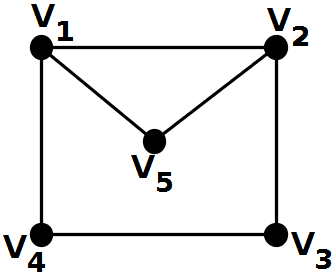
\includegraphics[width=3cm]{./img/envelope.png} & 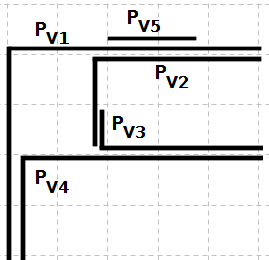
\includegraphics[width=4cm]{./img/envelopeHellyGradeTransparente.png} & 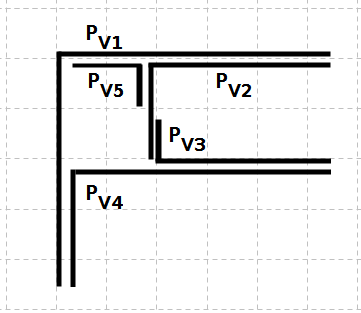
\includegraphics[width=4.6cm]{./img/envelopeNaoHellyGrade.png}
    \\
    \footnotesize \centering (a) Um grafo com  5 vértices & \footnotesize(b) Uma representação $B_1$-EPG que satisfaz a propriedade Helly & \footnotesize (c) Uma representação $B_1$-EPG que não satisfaz a propriedade Helly  \\

  \end{tabular}
\caption{Um grafo com 5 vértices em (a) e algumas representações de dobra simples: uma representação Helly em (b) e outra representação que não satisfaz a propriedade Helly em (c)} \label{fig:envelopeRepresentacoes}
\end{figure}



\subsection{O estudo de grafos EPG}

Um problema relacionado ao estudo de grafos EPG 
%Anterior ao estudo de grafos EPG existiu um problema similar, 
 é o problema de grafos de aresta-intersecção de caminhos em uma árvore, bem conhecido na literatura como EPT (Edge-intersection Graphs of Paths
in a Tree), ver~\cite{golumbic2004recognition}. Para grafos EPT, em particular, é resultado conhecido o valor dos parâmetros número de Helly, que  é 2, e do número de Helly forte, que é 3, resultados também em~\cite{golumbic2004recognition}. %A pesquisa de grafos EPG pode ser vista como uma extensão ao estudo pregresso de grafos EPT.

A respeito da complexidade do reconhecimento de grafos $B_k$-EPG, somente a complexidade de reconhecimento de três dessas subclasses de grafos foram determinadas: grafos
 $B_0$-EPG podem ser reconhecidos em tempo polinomial, uma vez que correspondem aos grafos de intervalo, ver~\cite{booth1976}. Em contraste, o reconhecimento de grafos $B_1$-EPG e $B_2$-EPG são problemas  $NP$-completos, ver~\cite{heldt2014, martin2017}, e o problema de reconhecimento de grafos $B_1$-EPG permanece $NP$-completo mesmo para caminhos $L$-shaped em grade, ver~\cite{cameron2016edge}.

Neste trabalho vamos estudar grafos que possuem uma representação EPG-Helly. Provamos que o problema de reconhecimento de grafos  $ B_1$-EPG-Helly é $NP$-completo. A propriedade Helly relacionada a representações de grafos EPG foi estudada por~\cite{golumbic2013} e~\cite{golumbic2009}. Em particular, eles determinaram o parâmetro  número de Helly forte de grafos $B_1$-EPG. 


 A pesquisa envolvendo grafos de aresta-intersecção de caminhos em grade é tópico relativamente novo na área de Teoria dos Grafos. As primeiras definições formais do problemas e aplicações foram apresentadas por Golumbic em 2009~\cite{golumbic2009}. Desde então diversas pesquisas têm sido conduzidas pela comunidade científica. Essas questões frequentemente abordam as representações dos caminhos, restrições quanto ao número de dobras em uma representação, entre outros. A seguir apresentaremos alguns trabalhos que conseguiram delimitar o \textit{número de dobras} para algumas classes de grafos.

No estudo de \citeauthor{alcon2016}, em~\cite{alcon2016}, os autores mostram que 3 dobras são suficientes para representar todos os grafos da classe de grafos arco-circular, i.e. eles estão em $B_3$-EPG. Adicionalmente, também mostram que existem grafos arco-circular que não podem ser representados com 2 dobras. Utilizando-se do fato de poder representar qualquer grafo arco-circular utilizando apenas um retângulo de uma grade de tamanho qualquer, o trabalho define a classe de grafos EPR e classificam os grafos arco-circular normais como sendo $B_2$-EPR, mostram ainda que existem grafos arco-circular normais que não são $B_1$-EPR. Finalmente, o trabalho dá uma caracterização de grafos $B_1$-EPR por uma família minimal de subgrafos induzidos proibidos e mostram que essa subfamília corresponde à uma subclasse de grafos normal arco-circular-Helly.

No trabalho de~\citeauthor{biedl2010}~\cite{biedl2010}, os autores mostram que 5 dobras são suficientes para representar todos os grafos planares e que 3 dobras são suficientes para representar todos os grafos outerplanar. Esses  resultados são posteriormente melhorados pelo trabalho de~\cite{daniel2014b}. Além desses resultados, o trabalho mostra que todo grafo planar bipartido possui representação EPG com 2 dobras e que todo grafo linha possui representação com 2 dobras. 


\citeauthor{daniel2014b} em~\cite{daniel2014b} mostraram que 4 dobras são suficientes para representar todos os grafos planares  e apresentam um algoritmo linear para encontrar essa representação com 4 dobras. Todavia, os autores ainda comentam que para alguns grafos planares, muitas vezes 3 dobras são suficientes para construção da representação. De fato, não é que simplesmente a maioria dos grafos planares poderiam ser construídos com 4 dobras, na verdade não se conhecem grafos planares que não podem ser desenhados utilizando apenas 3 dobras.   Isso deixa a seguinte questão: se 4 dobras são sempre suficientes para representar qualquer grafo planar então realmente são necessárias 4 dobras para representar qualquer grafo planar? Essa questão ainda está em aberto. Os autores ainda conjecturam que exista algum grafo onde para qualquer de suas representações EPG sempre existe pelo menos um caminho que precise utilizar as 4 dobras.

A Tabela~\ref{tab:limitesBenNumber} apresenta os principais limites conhecidos para o \textit{número de dobras}, notado como $b(G)$, de algumas classes de grafos.  


\begin{table}[h]
\caption{Algumas classes de grafos e limites conhecidos para o \textit{número de dobras}}
\label{tab:limitesBenNumber}
\begin{center}
\begin{tabular}{|c|c|c|}
\hline 
Classe de Grafo & b(G) & Referência \\ 
\hline \hline  
Grafos de Intervalo & 0 & \cite{golumbic2009} \\ 
\hline 
Florestas & 1 & \cite{golumbic2009} \\ 
\hline 
Outerplanar &  2 & \cite{daniel2014b} \\ 
% \hline 
% Planar & 5 e dim $(n-1)\times(2n-3)$ & \cite{biedl2010} 2010\\ 
\hline 
Planar & $\in [3, 4]$ & \cite{daniel2014b}\\ 
\hline  
Bipartido Planar & 2 & \cite{biedl2010} \\ 
\hline 
Grafo Linha & 2 & \cite{biedl2010} \\ 
\hline 
dgn(G)~\footnote{Degeneracy} $\leq k$ & $2k-1$ & \cite{daniel2014b} \\ 
\hline 
tw(G)~\footnote{Treewidth} $\leq k$ & $2k-2$ & \cite{daniel2014b} \\ 
\hline 
Degree $\leq \Delta$ & $ \in [	\lceil \frac{\Delta}{2}\rceil, \Delta ] $ & \cite{daniel2014b} \\ 
\hline 
Arco-circular & 3 & \cite{alcon2016} \\ 
\hline 
Normal Arco-circular & 2 & \cite{alcon2016} \\ \hline 
\end{tabular} 
\end{center}
\end{table}

Além dos resultados citados para limites do número de dobras de algumas classes de grafos, existem muitos trabalhos que caracterizam outros tipos de grafos não citados nessa tabela, como o trabalho de~\citeauthor{ries2009}~\citep{ries2009} que caracteriza os grafos cordais, livres de garra, touro e diamante que possuem uma representação $B_{1}$-EPG. Nesse mesmo artigo há também uma caracterização de alguns grafos split, com restrição ao tamanho do conjunto independente ou da clique, por subgrafos proibidos. O trabalho ainda tem um resultado interessante que mostra que a vizinhança de todo vértice de um grafo $B_1$-EPG induz um grafo fracamente cordal.

Apesar de ser possível encontrar várias pesquisas em grafos EPG investigando o número de dobras, os interesses de estudos nessa classe de grafos se estendem a outros problemas clássicos, os quais podemos citar a seguir.

Em~\citet{cohen2014} é apresentado um algoritmo de reconhecimento de tempo linear para cografos $B_{1}-$EPG por uma família de subgrafos induzidos proibidos. O algoritmo que o trabalho apresenta utiliza a co-árvore do cografo no processo de reconhecimento.
 
 Algoritmos aproximativos para coloração de grafos $B_1$-EPG foram estudados em~\cite{epstein2013approximation}. O trabalho citado mostra que o problema de coloração e o problema de conjunto independente máximo são ambos $NP$-completos para grafos $B_1$-EPG mesmo quando a representação EPG é dada. Os autores apresentam um algoritmo  4-aproximativo que resolve ambos os problemas, assumindo que a representação EPG é dada. O trabalho ainda mostra que a clique máxima pode ser encontrada de forma eficiente em grafos $B_1$-EPG mesmo quando a representação não é dada.
 
 Problemas de clique-coloração em grafos $B_1$-EPG foram estudados por~\cite{bonomo2017clique}. Os autores consideram o problema de clique coloração e mostram que grafos $B_1$-EPG são 4-clique-coloríveis e apresentam um algoritmo de tempo linear para resolver o problema.

Além dos trabalhos citados podemos mencionar também como pesquisa frequente com relação aos grafos EPG o estudo de complexidade \cite{daniel2014b, martin2017}, área da grade necessária para representação de um grafo cujo grau máximo é $\Delta(G)$ \cite{Asinowski2009}, e muitos outros.

Dentre os diversos temas estudados é possível perceber que a pesquisa que relaciona grafos EPG cujas representações satisfazem a propriedade Helly é escassa.
A dificuldade de reconhecimento de pouquíssimas classes de grafos EPG é conhecida, e ainda para valores de $k$ pequenos somente.  %Dessa forma, diante das aplicações apresentadas e dos trabalhos levantados na revisão da literatura, é possível perceber que pelo menos uma das propostas deste trabalho, que é investigar a dificuldade de reconhecimento de grafos $B_1$-EPG-Helly, é viável e factível do ponto de vista prático. Logo, 
 No capítulo seguinte nos dedicaremos a expor os principais resultados obtidos até aqui.

%\cite{Asinowski2009} mostrou que não existe um k para o qual todo grafo é B_k-EPG, somente uma quantidade exponencial de grafos pertencem a B_k-EPG para algum k dado.
  \chapter{A propriedade Helly e grafos EPG}\label{cap:capiii}

\begin{flushright}
\begin{minipage}[t][0cm][b]{0.47\textwidth}
\emph{
Talento é 1\% inspiração e 99\% transpiração. }
\end{minipage}

\rule[0cm]{7cm}{0.03cm}%{largura}{espessura}

Thomas Edison
\end{flushright}

Neste capítulo examinaremos as relações hierárquicas entre algumas classes EPG e EPG-Helly. Ademais, abordaremos representações $B_1$-EPG de alguns grafos que serão utilizados posteriormente. Primeiro, vamos observar como as classes $B_0$-EPG, $B_0$-EPG-Helly, $B_1$-EPG e $B_1$-EPG-Helly se relacionam, em seguida consideramos as representações $B_1$-EPG de $C_4$'s e do grafo octaedro. Por último, apresentaremos a prova de $NP$-completude do problema de reconhecimento de grafos $B_1$-EPG-Helly.


\section{Hierarquia de algumas classes EPG}

Apesar das classes $B_1$-EPG e $ B_1$-EPG-Helly não coincidirem,  o mesmo não ocorre para as classes $ B_0$-EPG e $ B_0$-EPG-Helly, conforme será visto mais adiante.

Primeiro, observamos que quando não restringimos o número de dobras de cada caminho podemos mostrar que qualquer grafo pode ser representado como um grafo EPG.
É fácil construir representações EPG que verificam o seguinte lema. 

 
 
 \begin{lema} \cite{golumbic2009} \label{lem:todoGrafoEpg}
 Todo grafo é um grafo EPG.
 \end{lema}
%   \begin{prove}
%  Seja $G=(V,E)$ um grafo com vértices $v_1,\dots ,v_n$. Considere a grade $Q$ com linhas $[1,\dots ,n]$ e colunas $[1, 1', 2, 2', \dots, n,n']$. 
 
%  Considere o vértice $v_i$ e denote $N^+(v_i)$= $\{v_j|i<j,(i,j)\in E\}$, onde $N^+(v_i)$= $\{v_{j_1}, \dots, v_{j_k}\}$ é ordenado de acordo com $\{v_{j_1}< \dots < v_{j_k}\}$.   The path $P_i$ on $Q$ is defined starting horizontally from grid point $(1,i)$ to $(i,i)$, continuing vertically to $(i,j_1)$, horizontally to $(i',j_1)$, continuing vertically to $(i,j_2)$, horizontally to $(i',j_2)$, continuing vertically $(i,j_3)$, horizontally $(i',j_3)$, etc. i.e., we alternate between column $i$ and column $i'$ as we go across on each level $j_1, j_2, \dots, j_k$. %reference Figure
%  We prove that $P_i$ on the grid $Q$ is an EPG representation of $G$. For every $i<j,(v_i,v_j)\in E(G)$ if and only if the paths $P_i$, $P_j$ contain the horizontal grid edge $((i,j), (i',j))$. Moreover, no paths share vertical grid edges. Therefore the vertices in the graph are adjacent if and only if the corresponding paths share a common grid edge.
%  $\square$ \end{prove}
 
 %Moreover, the same applies to EPG-Helly graphs. 
 
 De forma equivalente, também é possível mostrar que todo grafo possui uma representação EPG que satisfaz à propriedade Helly. Um algoritmo que efetua essa construção é apresentado no Lema~\ref{lem:todoGrafoEpgHelly}.
 
 \begin{lema}\label{lem:todoGrafoEpgHelly}
 Todo grafo é um grafo EPG-Helly.
 \end{lema}
%  \setcounter{prove}{1}
  \begin{proof}
  Seja $G$ um grafo com $n$ vértices $v_1, v_2, \dots, v_n$ e $\mu$ cliques maximais $C_1, C_2, \dots , C_{\mu }$. É possível construir uma representação EPG-Helly de $G$ usando uma grade $Q$ de tamanho $(\mu \times 2n)$. As linhas correspondem às cliques maximais e são enumeradas $1, 2, \dots , \mu$. Cada vértice $v_j$ corresponde ao par de colunas $j, j+n$. Cada clique maximal  $C_i$ é mapeada para uma aresta $(i,n), (i,n+1)$. %Cada caminho $P_j$ contém todas arestas $(i,n), (i,n+1)$ correspondendo às cliques maximais $C_i$ contendo $v_i$.
  
  %Além disso, dois caminhos distintos $P_j,P_k$ intersectam nas arestas correspondendo às cliques maximais contendo $v_j,v_k$.
  
  Tome $v_j \in V(G)$, considere a clique maximal contendo $v_j$ em ordem ascendente de seus índices. O caminho $P_j$ representando $v_j$, inicia no vértice $(1,j)$ de $Q$ e desce na coluna $j$ até $(i,j)$, onde $C_i$ é a primeira clique contendo $v_j$ então $P_j$ dobra no vértice  $(i,j)$ e prossegue para a direita, atravessa a aresta $(i,n), (i,n+1)$ representando $C_i$. Então $P_j$ prossegue  sobre a linha $i$ até atingir o vértice  $(i, j+n)$, onde dobra novamente, descendo na coluna $j+n$ até atingir o vértice $(l,j), l>i$, onde $C_l$ está a próxima clique maximal contendo  $v_j$ onde ele dobra mais uma vez. O caminho prossegue a linha $l$, atravessando a aresta $(l,n),(l,n+1)$, e assim por diante, até que todas as arestas de $Q$ correspondendo às cliques maximais contendo $v_j$ terem sido atravessadas por $P_j$.   
  
Segue então que dois caminhos distintos, $P_j$ e $P_q$, intersectam-se exatamente nas linhas correspondendo às cliques maximais contendo ambos $v_j$ e $v_q$.  
  \end{proof}
 
 A Figura~\ref{fig:gradeDemonstracao} apresenta a grade $Q$ e o caminho $P_2$ correspondendo ao vértice $v_2 \in V(G)$, contendo as cliques maximais  $C_2, C_4$ e $C_5$ de $G$.
 
  \begin{figure}[htb]	
\center%6.3
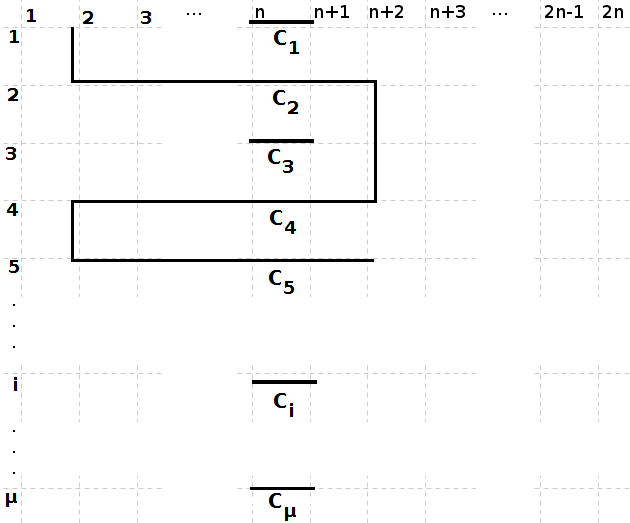
\includegraphics[width=8cm]{./img/grade3.png}
%clausulaGadgetGFCompletaSBPO
\caption{Representação do caminho $P_2$ correspondendo ao vértice $v_2$ contido nas cliques maximais $C_2, C_4$ e $C_5$}
\label{fig:gradeDemonstracao}
\end{figure}
 
 
 
 \begin{corollary}
 Todo grafo $G$ contendo  $\mu$ cliques maximais admite uma representação $B_{2\mu -1}$-EPG-Helly. %in a grid $Q$ of dimension $(\mu \times 2n)$.
 \end{corollary}
 

%Note que a classe de grafos $B_0$-EPG coincide com a bem conhecida classe de grafos de intervalo, i.e. grafos de intersecção de intervalos sobre uma reta real. 


\begin {lema} \label{lem:b0epg}
Toda representação $ B_0$-EPG satisfaz à propriedade Helly.
\end {lema}

\begin{proof}
Segue diretamente da seguinte observação de \citeauthor{golumbic2009}~\cite{golumbic2009}: a classe de grafos $B_0$-EPG pode ser vista como a classe de grafos de intervalo, grafos de intersecção de intervalos sobre uma linha. Note que  intervalos sobre linhas distintas da grade, horizontais ou verticais, formam componentes distintas do grafo.
\end{proof}


% \begin {proof}
% Assuma por contradição que exista um grafo $G$ que admite uma representação $ B_0$-EPG que não satisfaz à propriedade Helly. Então, essa representação possui uma coleção minimal de caminhos mutuamente intersectantes $ \mathcal{P} = \{P_{1}, P_{2}, \ldots, P_{k} \} $ tal que $ P_{1} \cap P_{2} \cap \cdots \cap P_{k} = \emptyset, k \geq 3. $
% Por minimalidade, sabemos que  $ \bar{P_1} = \mathcal{P} \setminus \{P_1 \}$, $ \bar {P_2} = \mathcal{P} \setminus \{P_2 \} $ e $ \bar {P_3 } = \mathcal{P} \setminus \{P_3) \} $ são mutuamente intersectantes e satisfazem à propriedade Helly.
% Assim, existem os seguintes segmentos distintos $ s_{\bar{P_1}}, s_{\bar {P_2}}, s_{\bar {P_3}}$ associados com a intersecção de caminhos em $ \bar {P_1},  \bar {P_2} $ e $ \bar {P_3} $. Uma vez que a representação não possui caminhos com dobras, então sabemos que os caminhos em  $ \mathcal{P}$ estão sobre a mesma linha.
% Sem perda de generalidade, vamos assumir que  $ s_{ \bar {P_1}}, s_{ \bar {P_2}}$ e $ s_{ \bar {P_3}}$ ocorrem da esquerda para a direita nessa ordem. Uma vez que $ s_{\bar {P_3}}$ e $ s_{\bar {P_1}}$ intersectam $ P_2 $, e $ P_2 $ é um caminho sem dobra, então $ P_2$ intersecta $ s_{\bar {P_2}}$. Dessa forma temos uma contradição, pois $ s_{\bar {P_2}} $ intersecta todos os caminhos em $ \mathcal{P}$, contradizendo a hipótese de $ P_1 \cap P_2 \cap \cdots \cap P_k = \emptyset $.
% \end {proof}
%%%%%%%%%

\begin{corollary}
A classe $B_0$-EPG coincide com a classe $B_0$-EPG-Helly.
\end{corollary}

Grafos $B_0$-EPG coincidem com a classe de grafos de intervalo. O problema de reconhecimento de grafos de intervalo pode ser resolvido em tempo linear~\cite{booth1976}. Já o problema de reconhecimento de grafos $ B_1$-EPG é $NP$-completo \cite {heldt2014}. Em particular, os grafos $ B_1$-EPG-Helly formam uma subclasse propriamente contida em $ B_1$-EPG, ver a Figura~\ref{fig:diagramaEPG}. Além disso, a complexidade de reconhecimento da classe de grafos $ B_1$-EPG-Helly é um problema em aberto. Este trabalho se propõe a resolvê-lo.% que foi resolvido por este trabalho. 

%O Lema \ref{lem:octaedronaohelly} mostra que 
As classes  $ B_1$-EPG e $ B_1$-EPG-Helly são distintas, observe o grafo octaedro $ O_3$, ver Figura~\ref{fig:octaedro}(a), que apresenta uma representação  $B_1$-EPG minimal, a menos de isomorfismos, como na Figura~\ref{fig:octaedro}(b). O grafo octaedro  $ O_3 $ pertence a $ B_1$-EPG mas não pertence a $B_1$-EPG-Helly.

\begin{figure}[htb]	
\center%6.3
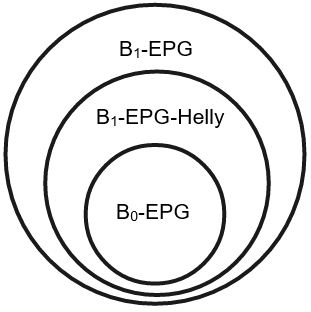
\includegraphics[width=3.5cm]{./img/diagramaClassesEPG.png}
\caption{Diagrama hierárquico de algumas classes  EPG}
\label{fig:diagramaEPG}
\end{figure}



\section{Representações $B_1$-EPG para os grafos $C_4$ e Octaedro}
%{The Classes $B_1$-EPG and $B_1$-EPG-Helly}

A seguir descrevemos quais são as representações de um grafo $C_4$ em uma representação de dobra simples. Uma descrição alternativa das possíveis representações de um $C_4$ pode ser encontrada em~\cite{golumbic2009}, onde o autor demonstra que são somente essas as poucas representações possíveis para o ciclo induzido de tamanho 4.


%By the results of \cite{golumbic2009}, in Lemma ~\ref{lem:representacaoC4}, every induced cycle of size 4 in a $ B_1$-EPG  representation  of $C_4$ has only a few possible representations.

\begin{definition} \label{defi:tortasFrame}

Seja $ Q $ uma grade e sejam $ (a_1, b),$ $(a_2, b),$ $(a_3, b),$ $(a_4, b)$ arestas que formam uma 4-estrela como retratado na Figura~\ref{fig:piesInGrid}(a). Seja  $ \mathcal{P} = \{P_1, \dots , P_4\}$ uma coleção de caminhos, cada um contendo exatamente duas arestas da $4$-estrela, definimos:

\begin{itemize}
\item Uma \emph{torta verdadeira} é uma representação onde cada caminho $P_i$ de $ \mathcal{P} $ forma uma dobra em $b$.

\item Uma \emph {torta falsa} é uma representação onde dois caminhos distintos $P_i, P_j$  não contém dobra, enquanto os dois caminhos restantes não compartilham aresta. 


\begin{figure}[htb]
  \centering
%segundo bloco de figuras
  \begin{tabular}{c c c c c }
    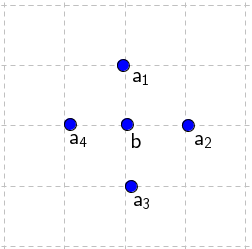
\includegraphics[width=3.5cm]{./img/disposicaoTortaGrid.png}    
    & &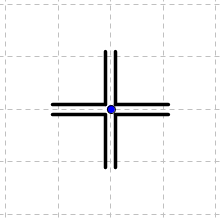
\includegraphics[width=3.5cm]{./img/truePieGrid.png} 
    & &
 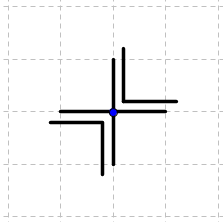
\includegraphics[width=3.5cm]{./img/falsePieGrid.png} \\%[\abovecaptionskip]
    {\footnotesize (a) 4-estrela na grade}  & &  {\footnotesize (b) Torta verdadeira} & & {\footnotesize (c) Torta falsa} %\label{fig:frame}
  \end{tabular}
  \caption{Representações $B_{1}$-EPG do ciclo induzido de tamanho  4 como tortas, com ponto central $b$}\label{fig:piesInGrid}
\end{figure} 

\end{itemize}
\end{definition}
%In both cases the point $b$ is called \emph{centro}, see Figures~\ref{fig:piesInGrid}(b) and~\ref{fig:piesInGrid}(c). There are edge-intersections $ (a_1, b), (a_2, b), (a_3, b), (a_4, b)$ called \emph{raio centrals}, see Figure~\ref{fig:piesInGrid}.

\begin{definition} \label{defi:tortasFrame2}
 Considere um retângulo de qualquer tamanho com os quatro cantos nos vértices  $ (x_1, y_1);$ $(x_2, y_1);$ $(x_2, y_2);$ $(x_1, y_2)$, posicionado como na Figura~\ref{fig:frameInGrid}. Uma \emph{moldura} é uma representação contendo os 4 caminhos de $\mathcal{P} =  \{ P_1, \dots, P_4\} $, cada um deles tendo uma dobra em um canto diferente do retângulo, e tal que os subcaminhos $ P_1 \cap P_2, P_2 \cap P_3, P_3 \cap P_4, P_4 \cap P_1 $, compartilham no mínimo uma aresta. Enquanto os subcaminhos  $ P_2 \cap P_4 $ e $ P_1 \cap P_3 $ não compartilham aresta.

\begin{figure}[htb]
  \centering
%segundo bloco de figuras
  \begin{tabular}{c c c c c }
    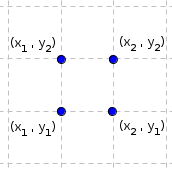
\includegraphics[width=3.5cm]{./img/dispositionFrameInGrid.png}    
    %& &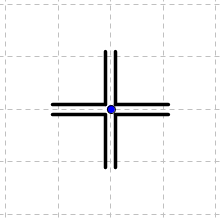
\includegraphics[width=4cm]{./img/truePieGrid.png} 
    & &
 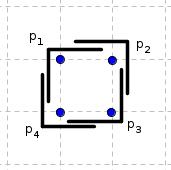
\includegraphics[width=3.5cm]{./img/frameInGrid.png} \\%[\abovecaptionskip]
    {\footnotesize (a) Pontos das coordenadas das dobras de uma moldura}  
    %& &  {\footnotesize (b) True pie} 
    & & {\footnotesize (c) Caminhos de uma moldura} %\label{fig:frame}
  \end{tabular}
  \caption{Representações $B_{1}$-EPG de um ciclo induzido de tamanho 4 por moldura} \label{fig:frameInGrid}
\end{figure} 
\end{definition}


%% \begin{figure}[htb]	
% \center%6.3
% 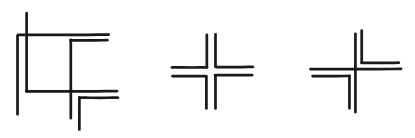
\includegraphics[width=10cm]{./img/representacaociclotam4.png}
% \caption{$B_{1}$-EPG representation of the induced cicle of size 4: frame (in left), true pie (center) and false pie (in right), \cite{golumbic2009}.}

% \end{figure}

\begin{figure}[htb]
  \centering
%segundo bloco de figuras
  \begin{tabular}{c c c c c }
    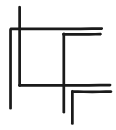
\includegraphics[width=2.3cm]{./img/representacaociclotam41.png}  
    & &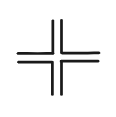
\includegraphics[width=2.5cm]{./img/representacaociclotam42.png} 
    & &
 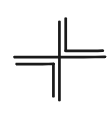
\includegraphics[width=2.5cm]{./img/representacaociclotam43.png} \\%[\abovecaptionskip]
    {\footnotesize (a) Frame}  & &  {\footnotesize (b) True pie} & & {\footnotesize (c) False pie} %\label{fig:frame}
  \end{tabular}
  \caption{$B_{1}$-EPG representation of the induced cycle of size 4}\label{fig:ciclotam4}
\end{figure} 


\begin{lema}\label{lem:representacaoC4}
\cite{golumbic2009} Todo $C_4$ que é um subgrafo induzido de um grafo $ G $ corresponde, em qualquer representação de dobra simples, a uma torta verdadeira, a uma torta falsa, ou a uma moldura.
\end{lema}
% \begin{prove} Consider a collection of paths $ P = \ {P_1, \dots, P_4}$ of a grid $ Q $ in a $ B_1$-EPG representation of the graph $G$.

% Consider $ C_4 = (v_1, v_2, v_3, v_4) $ that is a chordless 4-cycle in $ G$. Consider $P_i$ the path in $ G $ that corresponds to $v_i $.
% Suppose $ \displaystyle \bigcap _{P_i \in P} P_i \neq \emptyset $, then clearly $ \displaystyle \bigcap _{P_i \in P} P_i = {b} $, for some point $ b $ of the grid. Since each vertex in $ C_4 $ has exactly 2 neighbors, each path $ P_i $ contains exactly two edges of the grid with end point $ b$. Thus, we obtain a star subgraph with centro point $ b $ and edges $ (a_1, b), (a_2, b), (a_3, b), (a_4, b)$.
% Without loss of generality, $ P_1 $ contains the edges $ (a_1, b), (a_2, b) $ of the grid. If $ P_2 $ contains $ (a_2, b), (a_3, b) $ or $ (a_1, b), (a_4, b) $, then we get a torta verdadeira. Otherwise, $ P_2 $ contains the edges $ (a_2, b), (a_4, b) $ or $ (a_1, b), (a_3, b) $ and we obtain a torta falsa.

% Otherwise, $ \displaystyle \bigcaP_ {P_i \in P} P_i = \emptyset$. Suppose $ P_1 $ is a path without bend. Each of the $ P_2 $ and $ P_4 $ paths share an edge with $ P_1 $ but do not share a common edge with any other path. If $ P_2 $ and $ P_4 $ do not have a bend, then we get a interval representation of $ C_4 - v_3 $. However, it is not possible to add a $ P_3 $ path with at most of one bend. Similarly, if $ P_2 $ and $ P_4 $ have a single bend, the $ P_3 $ path can not be added either. Therefore, $ P_1 $ has a single bend.

% By symmetry, we assume that all $ P_i $ must has a single bend. Moreover, two paths can not have a bend on a common point in the grid. Thus, we obtain a rectangular subgraph with angles $ (x_1, y_1), (x_2, y_1), (x_2, y_2), (x_1, y_2) $, where $ P_1 $ bends at $ (x_1, y_1) $, $ P_2 $ bends at $ (x_2, y_1) $, $ P_3 $ bends at $ (x_2, y_2) $, and $ P_4 $ bends at $ (x_1, y_2) $, forming a frame.
% $\square$ \end{prove}

\begin{definition}
%A edge is \emph{unnecessary} if its removal keeps the intersections and not intersection of the representation. 
Uma representação $B_k$-EPG de um grafo $G$ é \emph{minimal} quando seu conjunto de arestas não contém propriamente outra representação $B_k$-EPG de $G$.
%when all unnecessary edges are removed.
\end{definition}

O grafo \textit{octaedro} é o grafo que contém  6 vértices e 12 arestas, retratado na  Figura~\ref{fig:octaedro}(a). A seguir, consideramos  representações do octaedro.

\begin{lema}\label{lem:octaedronaohelly}
O grafo octaedro  $O_3$ possui uma representação $ B_1$-EPG minimal única, a menos de isomorfismos.
\end{lema}
\begin{proof}
O grafo octaedro $ O_3 $ possui em sua constituição estrutural ciclos induzidos de tamanho  4 ($ C_4$'s). 
Tome um subgrafo $ C_4 $ qualquer do octaedro $ O_3$. O par de vértices não adjacentes do ciclo induzido são gêmeos falsos cuja vizinhança são os vértices pertencentes ao $C_4$ induzido. Cada vértice fora do $C_4$ é adjacente a todos os vértices do $C_4$. Assim quando a representação $ B_1$-EPG do $C_4$ é feita por  moldura, nenhum outro caminho da representação de dobra simples pode ser simultaneamente intersectante aos 4 caminhos da moldura. Portanto, concluímos que a estrutura moldura não pode ser parte de uma representação de dobra simples do grafo $ O_3$.

Com o mesmo raciocínio, tome uma representação $ B_1$-EPG de $C_4$ agora por torta verdadeira ou torta falsa. Quando adicionamos os caminhos correspondentes a vértices gêmeos falsos, de forma que sejam vizinhos a todos os vértices do $ C_4 $, obtemos $ O_3$, ambas representações convergem para a estrutura apresentada na Figura~\ref{fig:octaedro}(b). 
 \end{proof}

 \begin{figure}[h]
  \centering
  
%segundo bloco de figuras
  \begin{tabular}{@{}c@{} p{1.5cm} @{}c@{} }
   \centering 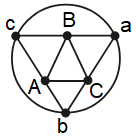
\includegraphics[width=2.5cm]{./img/octaedro.png} & &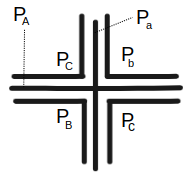
\includegraphics[width=4cm]{./img/representacaoOctaedro.png}  \\[\abovecaptionskip]
    \footnotesize \centering (a) O grafo octaedro $O_3$   & &  \footnotesize(b) Representação $B_1$-EPG do grafo $O_3$
  \end{tabular}

 \caption{O grafo octaedro $O_3$ e sua representação $B_1$-EPG}\label{fig:octaedro}
\end{figure}

Pelo Lema~\ref{lem:octaedronaohelly}, o grafo $ O_3 $ possui uma representação  $B_1$-EPG minimal única, a menos de isomorfismos, como retratado na Figura~\ref{fig:octaedro}(b). Como os caminhos $ P_a, P_b $ e $ P_c $  não satisfazem à propriedade Helly, então $O_3 \notin B_1$-EPG-Helly. 

\section{Pertinência a $\mathcal{NP}$}

%In this paper we are interested in characterizing the complexity of the $B_1$-EPG-Helly recognition problem, whose formal definition is presented next:
Nesta seção, mostraremos que o problema de reconhecimento de grafos $B_k$-EPG-Helly, onde $k$ é limitado por um polinômio de $|V(G)|$, pertence a  $\mathcal{NP}$. O problema pode ser formalmente descrito como segue.

\begin{table}[h!]
\centering
%\caption{My caption}
%\label{my-label}
\begin{tabular}{ll}
\hline \hline
\multicolumn{2}{c}{\sc Reconhecimento $B_k$-EPG-Helly}                         \\ \hline \hline 
\emph{Entrada}: & Um grafo $G$, e um inteiro $k$.\\
 & \\
\emph{Objetivo}: & \begin{tabular}[c]{@{}p{12.5cm}}
Determinar se existe um conjunto de caminhos $\mathcal{P} = \{P_1, P_2, \ldots, P_n\}$, com até $k$-dobras,  em uma grade  $ Q $ 
tal que: \\
\ \ $\bullet$ $v_i, v_j\in V(G)$ são adjacentes se e somente se  $P_i,P_j$ compartilham uma aresta em $Q$; \\
\ \ $\bullet$ $\mathcal{P}$ satisfaz à propriedade Helly.
\end{tabular} \\ \hline
\end{tabular}
\end{table}


Um certificado (positivo) para o problema {\sc Reconhecimento $B_k$-EPG-Helly} consiste de uma grade $Q$, um conjunto de caminhos $\mathcal{P}$ com até $k$-dobras sobre $Q$, que tenham uma correspondência de um-para-um com os vértices do conjunto $V(G)$ de $G$, tais que, para cada par de caminhos distintos $P_i, P_j\in \mathcal{P}, P_i\cap P_j \neq \emptyset $  se e somente se os vértices correspondentes são adjacentes em $G$. Além disso, $\mathcal{P}$ deve satisfazer à propriedade Helly.

Os seguintes conceitos são centrais para nosso propósito.
Uma \emph{aresta relevante} em uma representação $B_k$-EPG é aquela que é aresta de extremidade ou uma aresta de dobra. Portanto, como cada caminho possui no máximo $k$ dobras, então cada caminho pode ter até $2(k+1)$ arestas relevantes, e qualquer representação $B_k$-EPG contém no máximo $2|\mathcal{P}|(k+1)$ arestas relevantes.

%O certificado para o algoritmo de verificação que mostra que um grafo é um grafo $B_k$-EPG-Helly possui como parâmetros de entrada uma representação $B_k$-EPG, chamemos de $R$, contendo uma coleção de caminhos $\mathcal{P}$, $|\mathcal{P}|=|V(G)|$, onde cada caminho  $P_i \in \mathcal{P}$ é dado pelo seu conjunto de arestas relevantes mais o conjunto de arestas relevantes, que intersectam   $P_i$, de outros caminhos. As arestas relevantes devem ser dadas na ordem em que aparecem no caminho. Esse formato de codificação para os caminhos nos permite verificar se cada conjunto de arestas relevantes realmente representa um caminho com no máximo $k$-dobras. Essa representação também é útil para verificar se as intersecções correspondem a um modelo de intersecção para $G$.

%Um certificado (positivo) para  {\sc Reconhecimento $B_k$-EPG-Helly} consiste de uma grade $Q$, um conjunto  $\mathcal{P}$ de caminhos com $k$-dobras sobre $Q$, which have a one-to-one correspondence with the vertex set $V(G)$ of $G$, such that, for each pair of distinct paths $P_i, P_j\in \mathcal{P}, P_i\cap P_j \neq \emptyset $ if and only if the corresponding vertices are adjacent in $G$. Furthermore, $\mathcal{P}$ satisfies the Helly property.


Para mostrar que existe um algoritmo de tempo polinomial não determinístico para {\sc Reconhecimento $B_k$-EPG-Helly}, é suficiente considerar como certificado uma representação $B_k$-EPG, digamos  $R$, contendo uma coleção de caminhos  $\mathcal{P}$, onde $|\mathcal{P}| = |V(G)|$, tal que cada caminho   $P_i \in \mathcal{P}$  é dado pelo seu conjunto de arestas relevantes juntamente com o conjunto de todas as arestas relevantes de $P_j$ que intersectam $P_i$, onde $P_j \in \mathcal{P}$.  % as arestas relevantes, que intersectam $P_i$, de cada caminho $P_j$ que intersecta  $P_i$, onde $P_j \in \mathcal{P}$. 
 As arestas relevantes para cada caminho são dadas na ordem em que elas aparecem no caminho, de forma que é fácil checar se as arestas correspondem a um caminho único com no máximo  $k$ dobras. Essa representação é também utilizada para checar se os caminhos formam um modelo de intersecção para  $G$.

A fim de verificar, em tempo polinomial, que a entrada de fato é um certificado para o problema, temos que verificar as seguintes afirmações:

\begin{enumerate}[label=(\roman*)]
\item A sequência de arestas relevantes de um caminho $P_i\in \mathcal{P}$ determina unicamente $P_i$ em tempo polinomial; \label{it:bullet1}

\item Dois caminhos  $P_i, P_j \in \mathcal{P}$ são intersectantes se e somente se eles se intersectam em alguma aresta relevante; \label{it:bullet2}

\item O conjunto  $\mathcal{P}$ de arestas relevantes satisfaz à propriedade Helly. \label{it:bullet3}
\end{enumerate}

O Lema a seguir mostra que a condição~\ref{it:bullet1} é válida.

\begin{lema}\label{lem:verify1}
Cada caminho $P_i$ pode ser determinado unicamente, em tempo polinomial pela sua sequência de arestas relevantes.
\end{lema}

\begin{proof}
É fácil verificar que o item~\ref{it:bullet1} é verdadeiro. Considere a sequência de arestas relevantes de algum caminho $P_i\in \mathcal{P}$. Inicie de uma aresta de extremidade de $P_i$. Seja   $t$ a linha (coluna) contendo a última aresta relevante considerada. A próxima aresta relevante  $e'$ na sequência, deve estar contida na linha (coluna) $t$. Se $e'$ é uma aresta de extremidade, o processo está terminado e o caminho terá sido determinado. Ele contém todas arestas entre as arestas relevantes consideradas na sequência.  Caso contrário, se  $e'$ é uma aresta de dobra, a próxima aresta relevante é é a segunda aresta de dobra  $e''$ da mesma dobra, que está contida em alguma coluna (linha) $t'$. O processo continua até que a segunda aresta de extremidade de $P_i$ estar localizada.   

Com o procedimento acima podemos determinar em tempo $\mathcal{O}(k\cdot |V(G)|)$, se o caminho $P_i$ contém qualquer dada aresta da grade $Q$. Além disso, a sequência de arestas relevantes de  $P_i$ determina unicamente  $P_i$.
 \end{proof} %$\square$

O lema abaixo mostra que o item~\ref{it:bullet2} é válido.

\begin{lema}\label{lem:relevantEdges}
Seja $\mathcal{P}$ o conjunto de caminhos em uma representação $B_k$-EPG $R$ de $G$, e sejam $P_1,P_2 \in \mathcal{P}$. Então $P_1, P_2$ são caminhos intersectantes se e somente se sua intersecção contém no mínimo uma aresta relevante.%eles contêm no mínimo uma aresta relevante em comum.
\end{lema}

\begin{proof}
Se $P_1, P_2$ contém uma aresta relevante comum então claramente eles são intersectantes. Caso contrário, considere que $P_1, P_2$ são intersectantes, e mostraremos que eles contêm uma aresta relevante comum. Sem perda de generalidade, suponha que $P_1, P_2$ intersectam-se na linha \textit{i} da grade, em uma representação   $B_k$-EPG, digamos $R$. As seguintes são as possibilidades que podem ocorrer. 

Seja $e$ uma aresta comum a $P_1$ e $P_2$. Se $e$ não é aresta relevante, então a aresta seguinte à  esquerda (ou direita) de $e$, digamos $e'$, também pertence a $P_1 \cap P_2$. Tome $e'$, se $e'$ é relevante, então encontramos a aresta relevante da intersecção de $P_1$ e $P_2$, se não repetimos o processo até que uma aresta relevante seja encontrada. Caso os caminhos sejam juntos, uma aresta de dobra ou de extremidade é comum aos dois. Caso os dois caminhos se separem em algum ponto também existe uma aresta de dobra ou de extremidade que é comum aos dois.

% \begin{itemize}
% \item \textbf{Caso 1:} Nem $P_1$ nem $P_2$ contêm dobras na linha \textit{i}. 

% Então $P_1$ e $ P_2$  estão inteiramente contidos na linha \textit{i}. Uma vez que eles se intersectam, ou  $P_1, P_2$  se cobrem parcialmente, ou um dos caminhos contém o outro. Em qualquer dessas situações eles intersectam em uma aresta de extremidade comum, que é uma aresta relevante.

% \item \textbf{Caso 2:} $P_1$ não contém dobras em \textit{i}, mas $ P_2$ contém.

% Se alguma aresta de dobra de $P_2$ também pertence a   $P_1$, então $P_1, P_2$  intersectam-se em uma aresta relevante. Caso contrário, uma vez que $P_1, P_2$  intersectam-se, a única possibilidade é que a intersecção contenha uma aresta de extremidade de  $P_1$ ou $ P_2$. Portanto, os caminhos se intersectam em uma aresta relevante.

% \item \textbf{Caso 3:} Ambos $P_1$,  $P_2$ contém em \textit{i}.

% Novamente, se a intersecção ocorre em alguma aresta de dobra de $P_1$  ou $P_2$, o lema segue válido. Caso contrário,  a mesma situação anterior deve ocorrer, ou seja, $P_1, P_2$  devem intersectar em alguma aresta de extremidade.
 
% \end{itemize}
Em qualquer dos casos, $P_1$ e $P_2$ intersectam-se em alguma aresta relevante.
\end{proof}

Os dois lemas anteriores nos permitem checar que um certificado é uma representação $B_k$-EPG correta de um dado grafo $G$. O próximo lema diz que podemos verificar em tempo polinomial que a representação codificada em um certificado é uma representação Helly. Felizmente nós não precisamos checar todos os subconjuntos de caminhos intersectantes da representação para ter certeza que eles possuem uma intersecção comum.

Finalmente, provamos o item~\ref{it:bullet3}.


\begin{lema}\label{lem:verify3}
Seja $\mathcal{P}$ uma coleção de caminhos codificados como uma sequência de arestas relevantes que constituem uma representação $B_k$-EPG  de um grafo  $G$. Podemos verificar em tempo polinomial se $\mathcal{P}$  possui a propriedade Helly.
\end{lema}


\begin{proof}
Seja $\mathcal{T}$ o conjunto de arestas relevantes de $\mathcal{P}$. Consideramos cada tripla $T_i$ de arestas de  $\mathcal{T}$. Seja $\mathcal{P}_i$ o conjunto de caminhos de  $\mathcal{P}$ contendo no mínimo duas arestas relevantes de $T_i$. Pelo Teorema de Gilmore~\cite{bergeDuchet1975}, $\mathcal{P}$ possui a propriedade Helly se e somente se o subconjunto de caminhos de $\mathcal{P}_i$ correspondendo a cada tripla de $T_i$ tem intersecção não vazia.  Pelo Lema~\ref{lem:relevantEdges} é suficiente examinar a intersecção das arestas relevantes.  Além disso, um algoritmo polinomial para checar se $\mathcal{P}$ possui a propriedade Helly poderia examinar cada um dos subconjuntos $P_i$, e para cada aresta relevante $e$ de um caminho em $P_i$, computar o número de caminhos em $P_i$ que contêm $e$. $\mathcal{P}$ tem a propriedade Helly se e somente se para cada $P_i$ existe alguma aresta relevante que está em todos os caminhos de $P_i$ produzindo uma intersecção não vazia.
 \end{proof} %$\square$


\begin{corollary}\label{cor:comumAtodos}
Seja ${\mathcal P'}$ um conjunto mutuamente intersectante de caminhos em uma representação $B_k$-EPG-Helly de um grafo  $G$. Então a intersecção de todos os caminhos de ${\mathcal P'}$ contém no mínimo uma aresta relevante.
\end{corollary}

Note que a propriedade descrita no Corolário~\ref{cor:comumAtodos} é devida ao Teorema de Gilmore~\cite{bergeDuchet1975}, e se aplica somente a representações que satisfazem à propriedade Helly.

\medskip


\begin{lemma}\label{lem:gridPolinomial}
Seja $G$ um grafo $B_k$-EPG-Helly. Então $G$ admite uma representação $B_k$-EPG-Helly sobre uma grade de tamanho que é no máximo $4n(k+1) \times 4n(k+1)$.
\end{lemma}
\begin{proof}
Seja $R$ uma representação $B_k$-EPG de um grafo $G$ sobre uma grade $Q$ com o menor tamanho possível.
Seja $\mathcal{P}$ o conjunto de caminhos de  $R$. Note que $|\mathcal{P}|=n$.
 Existem no máximo $2|\mathcal{P}|(k+1)$ arestas relevantes em  $R$. 
 Se $Q$ possui um par de colunas consecutivas $c_i,c_{i+1}$ que não contém arestas relevantes de  $R$, e tais que não existem arestas relevantes cruzando de $c_i$ para $c_{i+1}$, então podemos contrair cada aresta cruzando de $c_i$ para $c_{i+1}$ em um único vértice de forma a obter uma nova representação  $B_k$-EPG  $G$ sobre uma grade de menor tamanho, o que é uma contradição. Um argumento análogo pode ser aplicado a pares de linhas consecutivas da grade.
  Portanto, a grade  $Q$ é tal que cada par de colunas consecutivas e de linhas consecutivas de  $Q$ tem no mínimo uma aresta relevante de $R$ ou contém uma aresta relevante cruzando-as.  
  Como $Q$ é a menor grade possível para representar  $G$ então a primeira linha e a primeira coluna de $Q$ ambas devem conter no mínimo um ponto  pertencendo a alguma aresta relevante de $R$. 
Assim, se $G$ é $B_k$-EPG então ele admite uma  representação $B_k$-EPG sobre uma grade de tamanho no máximo $4|\mathcal{P}|(k+1) \times 4|\mathcal{P}|(k+1)$.
Além do mais, pelo  Corolário~\ref{cor:comumAtodos}, sustenta-se que a operação de contração anteriormente descrita preserva à propriedade Helly, se houver. Assim, sendo $R$ uma representação $B_k$-EPG-Helly de um grafo $G$ sobre uma grade $Q$ com tamanho mínimo possível, é seguro afirmar que $Q$ possui tamanho no máximo  $4|\mathcal{P}|(k+1) \times 4|\mathcal{P}|(k+1)$.
\end{proof}

\begin{theorem}\label{teo:nppertinencia}
{\sc Reconhecimento $B_k$-EPG-Helly} está em  $\mathcal{NP}$, sempre que $k$ é limitado por uma função polinomial de $|V(G)|$.
\end{theorem}
\begin{proof}
Pelo Lema~\ref{lem:gridPolinomial} e o fato de que $k$ é limitado por uma função polinomial de  $|V(G)|$, segue que a coleção  $\mathcal{P}$ pode ser codificada através de suas arestas relevantes com   $n^{\mathcal{O}(1)}$ bits.

Finalmente, pelos Lemas~\ref{lem:verify1}, \ref{lem:relevantEdges} e \ref{lem:verify3}, segue que podemos verificar em tempo polinomial sobre o tamanho de $G$ se $\mathcal{P}$ é uma família de conjuntos codificada como uma sequência de arestas relevantes que constituem uma representação $B_k$-EPG-Helly de um grafo  $G$.
\end{proof}

\section{$NP$-Dificuldade}\label{sec:sectionDispositivoClausula}

Agora provaremos que o reconhecimento de grafos   $B_1$-EPG-Helly é $NP$-completo. Para essa demonstração seguiremos o roteiro de prova de dificuldade traçado por~\cite{heldt2014}.  Estabelecemos a redução do problema {\sc Positive (1 in 3)-3SAT} definido como segue:

\begin{table}[h!]
\centering
%\caption{My caption}
%\label{my-label}
\begin{tabular}{ll}
\hline \hline
\multicolumn{2}{c}{\sc Positive (1 in 3)-3SAT}                                \\ \hline \hline 
\emph{Entrada}: & \begin{tabular}[c]{@{}p{12.5cm}@{}} Um conjunto $X$ de variáveis positivas; uma coleção $\mathcal{C}=\{C_1,C_2,\ldots,C_m\}$ de cláusulas sobre  $X$ tal que para cada $C_i\in \mathcal{C}$, $|C_i|= 3$.
\end{tabular} \\
 &  \\
\emph{Objetivo}:  & \begin{tabular}[c]{@{}l@{}} %@{}l@{}
Determinar se existe uma atribuição de valores para as variáveis em $ X $\\ de modo que toda cláusula em  $\mathcal{C}$ tem exatamente um literal verdadeiro.
\end{tabular} \\ \hline
\end{tabular}
\end{table}

{\sc Positive (1 in 3)-3SAT } é um problema $NP$-completo bem conhecido (ver \cite{johnson1979}, problema [L04], pág. 259). {\sc Positive (1 in 3)-3SAT} permanece $NP$-completo quando o grafo de incidência da fórmula CNF (Conjunctive Normal Form) é um grafo planar~\cite{mulzer2008minimum}.

Dada uma fórmula  $F$ que é uma instância de {\sc Positive (1 in 3)-3SAT} apresentaremos uma construção de tempo polinomial de um grafo $ G_F$ tal que  $ G_F $ é $ B_1$-EPG-Helly se e somente se $ F $ é satisfativa. Esse grafo conterá um subgrafo induzido  $ G_{c_i}$ com 12 vértices (chamado \emph {dispositivo cláusula}) para toda cláusula $C_i \in F$, e um subgrafo induzido (\emph {dispositivo variável}) para cada variável $ x_j$, contendo um vértice especial   $ v_j$, além de um  \emph{dispositivo base}  com 55 vértices adicionais.

%Since a Sun graph $S_4$ whose centro is a cycle of size 4 and adding a false twin to each vertex of $S_4$ that is not a member of central induced cycle then we have the graph $H$. 
Utilizaremos um grafo $H$ isomorfo ao grafo ilustrado na Figura~\ref{fig:gadgetBase}, como um  dispositivo para realizar a prova. Para cada cláusula  $C_i$ de $F$ do nosso problema alvo, teremos um \emph{dispositivo cláusula} isomorfo a $H$, denotado por $G_{C_i}$. %The graph $H$ consists of subgraphs whose $B_1$-EPG representations are well known, such as: cycles of sizes 3 and 4.

\begin{figure}[htb]	
\center%6.3
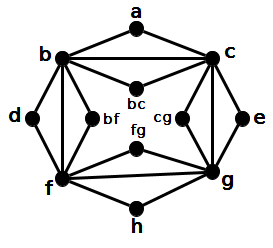
\includegraphics[width=5cm]{./img/gadgetBase.png}
\caption{O grafo dispositivo parcial $H$}
\label{fig:gadgetBase}
\end{figure} 

%\subsection{Definition}\label{sec:reducao}%The problem reduction}

A redução  de uma instância $F$ de  {\sc Positive (1 in 3)-3SAT}  para um grafo particular $G_F$ tal que $G_F$ possui uma representação $B_{1}$-EPG-Helly se e somente se $F$ é satisfatível, é dada abaixo.

\begin{definition}\label{sec:reducao}
Seja $F$ uma fórmula na CNF sem literais negativos, em que toda cláusula possui exatamente três literais. O grafo $G_F$ é construído como segue:

\begin{enumerate}
\item Para cada cláusula $C_i \in F$ criar um \textit{dispositivo cláusula} $G_{C_i}$, isomorfo ao grafo $H$;

\item Para cada variável $x_{j}$ criar um \emph{vértice-variável} $v_{j}$ que é adjacente aos vértices $a$, $e,$ ou $h$ de $G_{C_i}$, quando $x_{j}$ é a primeira, segunda ou terceira variável em $C_i$, respectivamente;

\item Para cada vértice-variável $v_{j}$, construir um \emph{dispositivo variável} formado pela adição de duas cópias de  $H$, digamos $H_1$ e $H_2$, e fazendo $v_j$ adjacente aos vértices do triângulo $(a, b, c)$ em  $H_1$ e $H_2$.

 %where $v_{j}$ is  adjacent to all vertices of the triangle (a,b,c);%; (c,e,g); (g,f,h); or (b,d,f)) of each $H_1$ and $H_2$; 

%\item The  subgraph induced by \emph{vértice-variável}  $v_{j}$, and also $V(H_1)$ and $V(H_2)$ will be called \emph{dispositivo variável}; 

\item Criar um vértice $V$, que será utilizado como referência vertical para a construção, e adicionar arestas de  $V$ para cada vértice  $d$ nos \emph{dispositivos cláusula};%$d \in V(G_c)$;

\item Criar um grafo bipartido $K_{2,4}$ com um vértice particular $T$ que faz parte do maior conjunto estável desse $K_{2,4}$. Esse vértice é denominado \emph{vértice-verdadeiro}. $T$ é adjacente a todos  $v_{j}$ e também a $V$;

\item Criar dois grafos isomorfos a $H$, digamos $G_{B1}$ e $G_{B2}$. O vértice $T$ é conectado a todos os vértices do triângulo $(a,b,c)$
em $G_{B1}$ e $G_{B2}$;


\item Criar dois grafos isomorfos a $H$, digamos $G_{B3}$ e $G_{B4}$. O vértice $V$ está conectado a todos os vértices do triângulo $(a,b,c)$ em $G_{B3}$ e $G_{B4}$;

\item O subgrafo induzido pelo conjunto de vértices $\{V(K_{2,4}) \cup  \{T, V\} \cup V(G_{B1}) \cup V(G_{B2}) \cup V(G_{B3}) \cup V(G_{B4})\}$ será denominado como \emph{dispositivo base}. 
\end{enumerate}
\end{definition}


A Figura~\ref{fig:exemploGrafoGF} retrata como essa construção funciona quando aplicada sobre uma pequena fórmula. %represents the graph that would be obtained when the previous construction is applied to the formula $ F = (x_1 + x_2 + x_3) \wedge (x_2 + x_3 + x_4) \wedge (x_3 + x_1 + x_4)$.


\begin{figure}[htb]	
\center%6.3
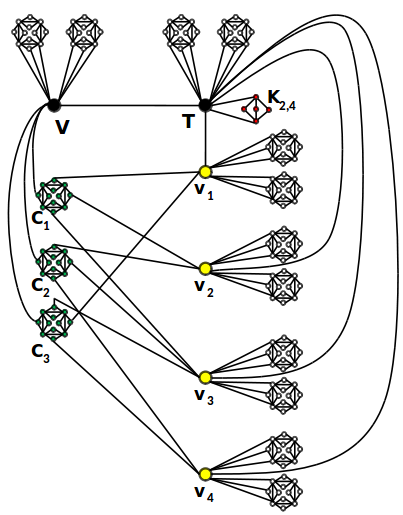
\includegraphics[width=6.5cm]{./img/exemploGrafoGFSBPO4.png}
\caption{O grafo $G_{F}$ correspondendo à fórmula $F=(x_1+ x_2+ x_3) \wedge  (x_2+ x_3+ x_4 )\wedge  (x_3 + x_1 + x_4 )$}
\label{fig:exemploGrafoGF}
\end{figure}


\begin{lema}\label{lem:ida}
Dada uma instância satisfatível $F$ de {\sc Positive (1 in 3)-3SAT}, o grafo  $G_F$ construído a partir de $F$ de acordo com a Definição~\ref{sec:reducao} admite uma representação $B_{1}$-EPG-Helly.
\end{lema}


\begin{proof}

%~\ref{fig:representacaoCaminhos}
Utilizaremos as estruturas  torta verdadeira e torta falsa para representar os  \textit{dispositivo cláusula} $ G_C$, mas a construção poderia ser feita com a estrutura moldura sem perda de generalidade, ver Figura~\ref{fig:falseAndTruePie}.  


\begin{figure}[htb]
  \centering
%segundo bloco de figuras
  \begin{tabular}{c c c }
    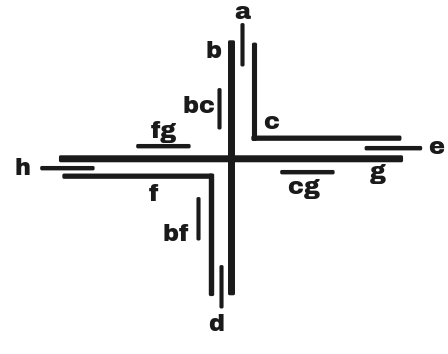
\includegraphics[width=4.5cm]{./img/falsePie.png}  %\label{fig:falsePie} 
    & &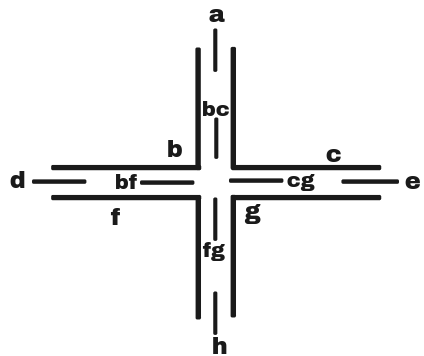
\includegraphics[width=4.5cm]{./img/truePie.png} %\label{fig:truePie}
    \\%[\abovecaptionskip]
    {\footnotesize (a) Baseado em torta falsa}  & &  {\footnotesize(b) Baseado em torta verdadeira}\\
  \end{tabular}
  \caption{Representação de dobra simples  de um dispositivo cláusula isomorfo ao grafo $H$} \label{fig:falseAndTruePie}
\end{figure} 

Os \textit{dispositivo variável} serão representados por estruturas como da Figura~\ref{fig:gadgetVariavel}.

\begin{figure}[htb]	
\center%6.3
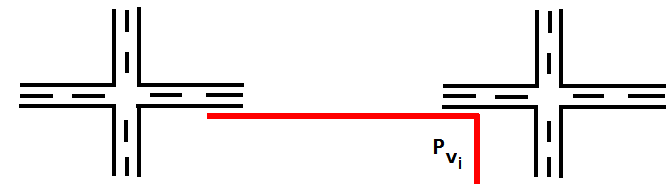
\includegraphics[width=10cm]{./img/gadgetVariavel.png}
%clausulaGadgetGFCompletaSBPO
\caption{Representação de dobra simples de um dispositivo variável}
\label{fig:gadgetVariavel}
\end{figure}


O \textit{dispositivo base} será representado pela estrutura retratada na  Figura~\ref{fig:gadgetBaseSingleBend}.

\begin{figure}[htb]	
\center%6.3
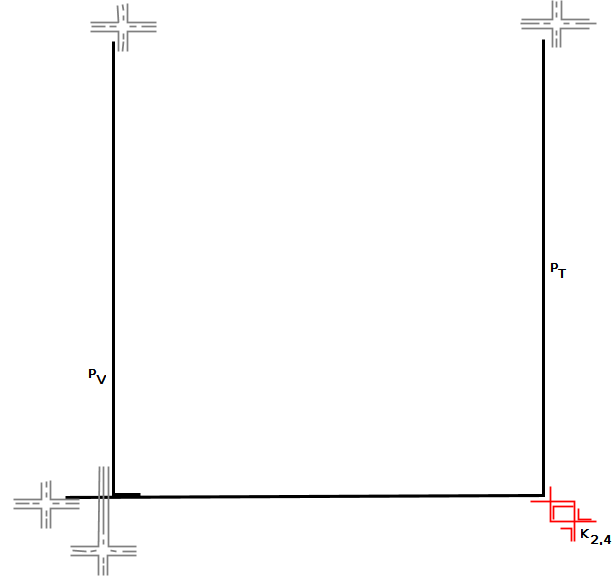
\includegraphics[width=10cm]{./img/gf2.png}
%clausulaGadgetGFCompletaSBPO
\caption{Representação de dobra simples do dispositivo base}
\label{fig:gadgetBaseSingleBend}
\end{figure}


É fácil ver que as representações dos dispositivo cláusula, dispositivo variável e dispositivo base são todas  $B_1$-EPG-Helly. Agora precisamos descrever como essas representações podem ser combinadas de forma a construir uma representação  de dobra simples $R_{G_F}$.

Dada uma atribuição  $A$ que satisfaz  $F$, podemos construir uma representação $R_{G_F}$ que seja  $B_{1}$-EPG-Helly. Primeiro, fixaremos a estrutura de representação do dispositivo base na grade para organizar a representação, ver Figura~\ref{fig:gadgetBaseSingleBend}. A seguir inserimos o  dispositivo variável com a seguinte regra: se a variável $x_i$ relacionada ao caminho   $P_{v_i}$ tiver atribuição  \textit{True}, então a adjacência entre o caminho $P_{v_i}$ com $P_{T}$ é horizontal, e vertical caso contrário. Por exemplo, uma atribuição  $A=\{x_1=False; x_2=False;x_3=True; x_4=False\}$  para as variáveis da fórmula  $F$ que gerou o dispositivo $G_F$ da Figura~\ref{fig:exemploGrafoGF}, nos dará um representação de dobra simples (dispositivo base + dispositivo variável) de acordo com a  Figura~\ref{fig:gadgetBasePlusVariables}(a). 

Quando a fórmula  $F$ de {\sc Positive (1-in-3)-3sat} possui cláusulas cujo formato de atribuição é $(False, True, False)$ ou $(False, False, True)$ então usaremos torta falsa para representar essas cláusulas, mas quando a cláusula tem formato  $(True, False, False)$ utilizaremos  torta verdadeira para representar essa cláusula. Para inserir um  \textit{ dispositivo cláusula} $G_{C_i}$, introduziremos uma linha horizontal $l_{h}$ na grade entre as linhas horizontais usadas pelos caminhos para as duas variáveis $False$ em $ C_i $. Então conectaremos o caminho $P_{d_{c_i}}$ de $G_{C_i}$ em $P_{V}$ verticalmente usando a dobra de  $P_{d_{c_i}}$. No entanto, introduziremos uma linha vertical $ l_{v}$, na grade, entre a linha vertical da grade usada por $P_{V}$ e o caminho para  a variável $True$ em $C_i$, i.e. entre $P_{V}$ e o caminho representando a variável  $x_j \in C_i$. Onde  $l_{h}$  e $l_{v}$ cruzarem, nesse ponto iremos inserir o centro do  \textit{dispositivo cláusula} como pode ser visto na Figura~\ref{fig:gadgetOnePie}(b). Uma construção completa dessa representação de dobra simples para  $G_F$ pode ser verificada na 
Figura~\ref{fig:gadgetFormulaCompletaPies}.%~\ref{fig:clausulagadgetgf}. 

\begin{landscape}
\begin{figure}[h]
  \centering
%segundo bloco de figuras
  \begin{tabular}{p{10cm} p{2cm} p{10cm}}
   \centering 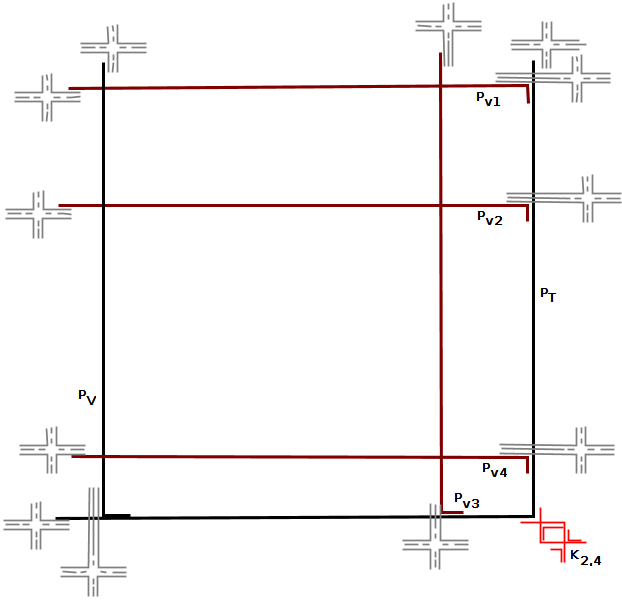
\includegraphics[width=10cm, left]{./img/gf3.png} & & 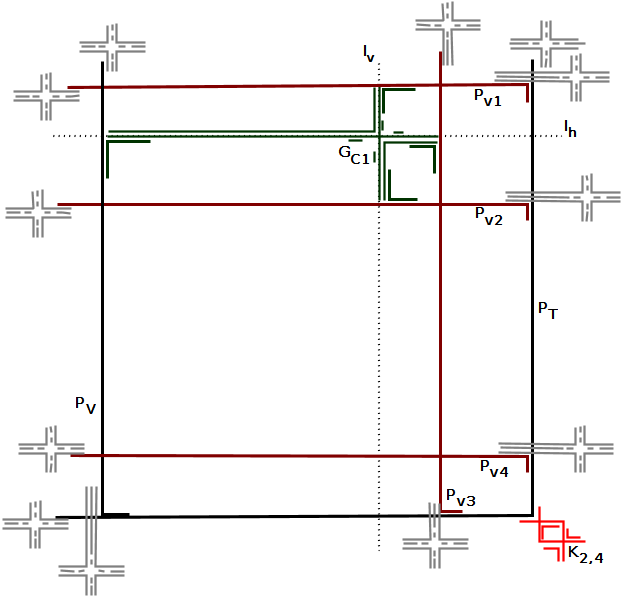
\includegraphics[width=10cm, left]{./img/formulaCompletaGFonePiePlusLines.png} \\  
  [\abovecaptionskip]
    \footnotesize \centering (a) Representação com dispositivos cláusula omitidos & & \footnotesize(b) Representação  com  $G_{C_1}$  associado com a cláusula $(x_1+x_2+x_3)$ em destaque \\
  \end{tabular}

 \caption{Representação de dobra simples dos dispositivos base e variáveis associados com as atribuições $x_1=False, x_2=False, x_3=True, x_4=False$} \label{fig:gadgetOnePie} \label{fig:gadgetBasePlusVariables}
\end{figure}
\end{landscape}


\begin{figure}[htb]	
\center%6.3
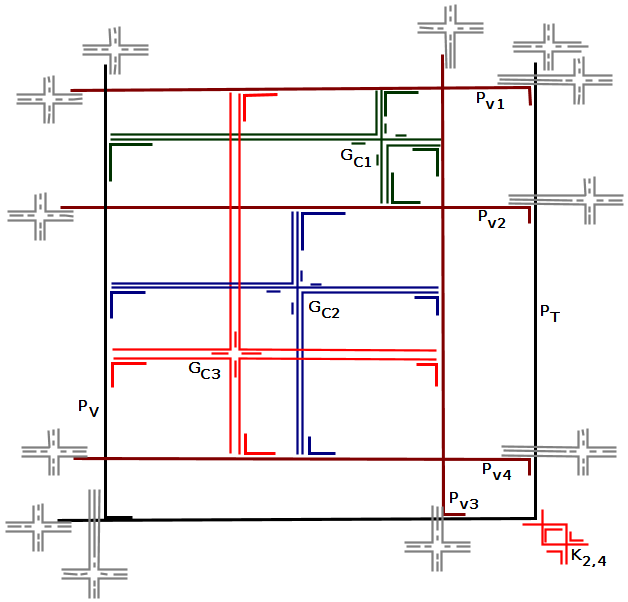
\includegraphics[width=10cm]{./img/formulaFGCompletaPies.png}
%clausulaGadgetGFCompletaSBPO
\caption{Representação de dobra simples de $G_F$}
\label{fig:gadgetFormulaCompletaPies}
\end{figure}


Note que quando juntamos todas essas representações  dos  dispositivos que formam $ R_{G_F} $ não há inserção de mais dobras nos caminhos que já possuíam dobra, então a representação necessariamente permanece sendo uma representação  $ B_1$-EPG válida. Nos resta mostrar que ela satisfaz à propriedade Helly. 

Uma forma simples de verificar que $ R_{G_F} $ satisfaz à propriedade Helly é notar que o grafo particular  $G_F$ nunca forma triângulos entre dispositivo variável, cláusula e base. Assim, qualquer triângulo de  $G_F$ está contido nos dispositivo variável, cláusula ou base. Como usamos somente representações  $B_1$-EPG-Helly desses dispositivos, $ R_{G_F} $ permanece uma representação $B_1$-EPG-Helly de $G_F$.
 \end{proof}

%\cleardoublepage
%\newpage

A seguir consideramos a conversão. Tome uma representação $B_1$-EPG-Helly, $R$ de $G_F$.

%To complete the proof of $NP$-hardness we will  present some considerations related with the single bend representation of gadgets that form the graph $G_F$. The way all gadgets can be drawn makes it possible to recover the formula that generated $G_F$ and a $True-$assignment for it. The following proofs help us understand the construction of a representation to $G_F$.  

\begin{definition}
Seja $H$ o grafo mostrado na  Figura~\ref{fig:gadgetBase}, tal que um 4-ciclo $H[\{b, c, f, g \}]$ corresponde em $R$ a uma estrutura de torta falsa ou torta verdadeira, então:

\begin{itemize}
\item O \emph{centro} é o único ponto da grade dessa representação que está contido em todo caminho representando o 4-ciclo $ \{b, c, f, g \}$; \label{lab:lab1}

\item Um \emph {raio central} é uma aresta-intersecção entre dois dos caminhos correspondendo aos vértices $ b, c, f, g$, respectivamente.
\end{itemize}
\end{definition}


Note que toda representação $B_1$-EPG de um $C_4$ satisfaz à propriedade Helly, ver Lema~\ref{lem:representacaoC4}, e os triângulos possuem $B_1$-EPG representações que satisfazem à propriedade Helly, e.g. a retratada na Figura~\ref{fig:trianguloepgRepresentacao}(b). O grafo $H$ é composto por um 4-ciclo,  $C_4^{H}=H[b, c, f, g]$ e oito triângulos, que são $(a,b,c);$ $(b,c,bc);$ $(c,e,g);$ $(c,g,cg);$ $(f,g,h);$ $(f,g,fg);$ $(b,d,f);$ $(b,f,bf).$

Como $C_4^{H}$ é um grafo que possui representações bem conhecidas (ver Lema~\ref{lem:representacaoC4}), então podemos iniciar o desenho da representação $B_{1}$-EPG-Helly de $H$ dessas estruturas. As  Figuras~\ref{fig:falsepietruepieframe} retratam possibilidades de representações para $H$.

Se um $C_4^{H}$ é representado por torta verdadeira ou torta falsa, então os caminhos $P_b, P_c, P_f, P_g$ compartilham um ponto central da representação. Por outro lado, se  $C_4^{H}$ é representado por uma moldura então as dobras dos caminhos correspondem aos quatro cantos distintos de um retângulo, i.e. todos os caminhos representando  vértices de um $C_4^{H}$ possuem pontos de dobra distintos, ver~\cite{golumbic2009}.

A seguir examinaremos o uso da estrutura moldura.

%Due asymmetric representations, the moldura structure needs to be studied in more detail. Next we will show some constraints of this structure. % in which allow us to consider it. %as gadget in the demonstration.

\begin{proposition}\label{lem:direcoesdiferentes}
Em uma representação $B_1$-EPG de um $C_4$ isomorfa a uma moldura, todo caminho  $P_i$ que representa um vértice do $C_4$ intersecta exatamente dois outros caminhos $P_{i-1}$ e $P_{i+1}$ da moldura, de modo que uma das intersecções é vertical e a outra é horizontal. %where one of them is vertical and another is a horizontal intersection.
\end{proposition}

\begin{proof}
A prova é imediata, pela definição de moldura.
 \end{proof}

\begin{proposition}\label{lem:mesmaretasuporte}
Dada uma representação $B_1$-EPG-Helly de um grafo $G$ que possui um $C_4$ induzido cuja representação é isomorfa a uma moldura. Se existe um vértice $v$ de $G$, fora desse $C_4$, que é adjacente a exatamente dois vértices consecutivos desse $C_4$, então o caminho representado por  $v$ possui uma aresta comum com os caminhos representando ambos vértices do $C_4$.% of $v$ into such .  
\end{proposition}

\begin{proof}
Por suposição, $G$ possui um triângulo contendo  $v$ e dois vértices de um $C_4$ representado por moldura. Além disso, o caminho representando  $v$ compartilha no mínimo uma aresta que é intersectante aos caminhos que representam seus vizinhos, caso contrário a representação não satisfaz à propriedade Helly.
 \end{proof}

%\cleardoublepage

Pela Proposição~\ref{lem:direcoesdiferentes} e Proposição~\ref{lem:mesmaretasuporte} podemos concluir que para todo vértice   $v_i \in V(H)$ tal que $v_i \neq V(C_4^{H})$, quando usamos uma moldura para representar o $C_4^{H}$, $P_{v_i}$ terá no mínimo uma aresta-intersecção comum ao par de caminhos representando seus vértices vizinhos em $H$. 
A Figura~\ref{fig:falsepietruepieframe}(c) retrata uma possível representação $B_{1}$-EPG-Helly de $H$. 
Note que ao aplicarmos operações de rotação e espelhamento, mantemos a representação $B_1$-EPG-Helly de $H$.
%On this $B_{1}$-EPG-Helly representation presented we can apply rotation and mirroring operations, because these operations do not change the structure. We can also a change the direction of the bend (see Figure~\ref{fig:falsepietruepieframe}(c) and Figure~\ref{fig:outraRepresentacaoFrame}), but also adjust other paths if needed, so as to not change the intersections between the paths.

\begin{definition}
Em uma representação de dobra simples de um grafo  $C_4$ isomorfo a uma moldura, os caminhos representando vértices consecutivos no  $C_4$ são chamados \emph{caminhos consecutivos} e o segmento que corresponde à intersecção entre dois caminhos consecutivos é chamado \emph{intersecção de lado}.  
\end{definition}

\begin{lema}\label{lem:2vertical2horizontal}
Em qualquer representação minimal de dobra simples de um grafo isomorfo a $H$, existem dois caminhos em   $\{P_a, P_e, P_d, P_h \}$ que tem direção horizontal e os outros dois caminhos possuem direção vertical.
\end{lema}

\begin{proof}
Se o $C_4^{H} = [b,c,f,g]$ é representado por uma torta verdadeira ou torta falsa então cada caminho do  $C_4^{H}$ compartilha dois raios centrais com dois outros caminhos do  $C_4^{H}$, onde cada raio central corresponde a um par de vértices consecutivos no $C_4^{H}$.

Como os vértices  $a, e, d, h$ são adjacentes a pares de vértices consecutivos no $C_4^{H}$ então os caminhos $P_a, P_e, P_d, P_h$ tem que se posicionar em cada um dos diferentes raios centrais,  2 estão na direção horizontal e 2 estão na direção vertical.

Se o $C_4^{H}$ é representado por uma moldura então cada caminho do $C_4^{H}$ possui uma dobra posicionada em uma curva da moldura. Na moldura, o relacionamento de adjacência de pares de vértices consecutivos no $C_4^{H}$ é representado pela intersecção dos caminhos que constituem a moldura. Assim, como uma moldura possui duas partes da direção vertical e duas partes na direção horizontal, então existem dois caminhos em $\{P_a, P_e, P_d, P_h\}$ que possuem direção vertical e dois caminhos que possuem direção horizontal.
 \end{proof}

\begin{corollary}
 \label{coro:paresMesmoSegmento}
Em qualquer representação minimal de dobra simples de um grafo isomorfo a $H$, os seguintes caminhos estão sobre o mesmo raio central ou intersecção de lado: %$P_a$ and $p(bc)$; $p(e)$ and $p(cg)$; $p(h)$ and $p(fg)$; $p(d)$ and $p(bf)$.

\begin{itemize}
\item $P_a$ e $P_{bc}$;
\item $P_e$ e $P_{cg}$;
\item $P_h$ e $P_{fg}$;
\item $P_d$ e $P_{bf}$.
\end{itemize}
\end{corollary}

\begin{figure}[htb]
  \centering
%segundo bloco de figuras
  \begin{tabular}{c c c c c }
    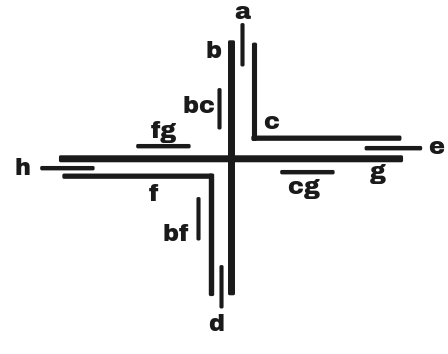
\includegraphics[width=4cm]{./img/falsePie.png}  %\label{fig:falsePie} 
    & &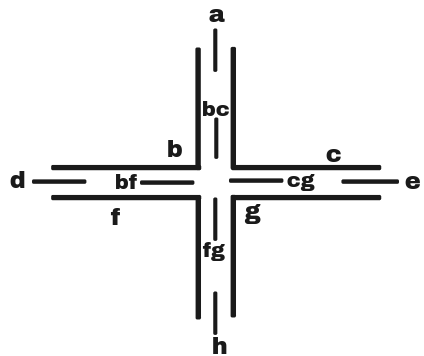
\includegraphics[width=4cm]{./img/truePie.png} %\label{fig:truePie}
    & &
 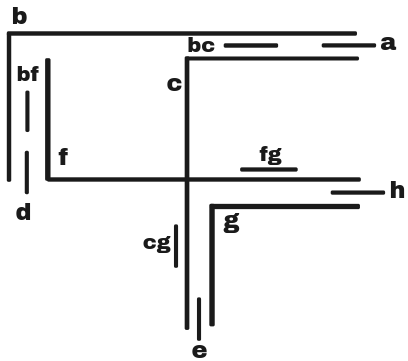
\includegraphics[width=4cm]{./img/frame.png} \\%[\abovecaptionskip]
    {\footnotesize (a) Baseada em torta falsa}  & &  {\footnotesize(b) Baseada em torta verdadeira} & & {\footnotesize (c) Baseada em moldura} %\label{fig:frame}
  \end{tabular}
  \caption{Diferentes representações de dobra simples para o grafo  $H$ utilizando uma  torta falsa (a), uma torta verdadeira (b) e uma moldura (c) para representar o $C_4^{H}$}\label{fig:falsepietruepieframe}
\end{figure} 

\begin{figure}[htb]	
\center%6.3
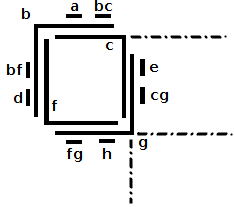
\includegraphics[width=4cm]{./img/outraRepresentacaoFrame3.png}
\caption{Uma representação por moldura onde as dobras dos caminhos pontilhados mudaram de sentido}
\label{fig:outraRepresentacaoFrame}
\end{figure}

\begin{definition}
Considere um grafo $G$ e um vértice $v \in V(G)$. Se em uma representação $B_1$-EPG de $G$ as duas arestas de dobra (ou uma aresta de extremidade) do caminho $P_v$ intersecta outros caminhos, então dizemos que  $P_v$ possui uma \emph{dobra obstruída (ou extremidade obstruída)}. 
Além do mais, dada uma representação $B_1$-EPG de $G$ onde $P_v$ possui uma dobra (ou extremidade) obstruída, dizemos que um subconjunto de caminhos \emph{obstrui} uma aresta de dobra (ou uma aresta de extremidade) de  $P_v$ se eles intersectam essa aresta. 
\end{definition}


\begin{fac} \label{fact:k24facts}
Em toda representação de dobra simples de um $K_{2,4}$, o caminho representando cada vértice do maior conjunto estável tem dobra em uma  torta falsa (ver mais em~\cite{Asinowski2009} e~\cite{daniel2014b}).
\end{fac}


\begin{lema}\label{lem:obstrucao}
Em qualquer representação de dobra simples do grafo  $G'$ retratado na  Figura~\ref{fig:extremidadeDobraObstruida}(a), o caminho $P_x$ possui extremidades e dobra obstruídos.
\end{lema}

\begin{proof}
Considere $G'$ consistindo de um vértice $x$, dois grafos isomorfos a  $H$, digamos $ H_1 $ e $ H_2 $, e um grafo bipartido $K_{2,4}$, tal que: $x$ é vértice do maior conjunto estável de $K_{2,4}$; $x$ é adjacente a um ciclo induzido de tamanho 3 de $H_1$, digamos $C_3^{H_1}$, e a um ciclo induzido de tamanho  3 de $H_2$, digamos $ C_3^{H_2}$, ver Figura~\ref{fig:extremidadeDobraObstruida}(a).

Sabemos que os caminhos pertencentes ao maior conjunto estável de um $K_{2,4}$ sempre dobram em uma  torta falsa, ver Fato~\ref{fact:k24facts}. Além disso $P_x$ é parte do maior conjunto estável desse  $K_{2,4}$, então $P_x$ possui uma \emph {dobra obstruída}, ver Figura~\ref{fig:extremidadeDobraObstruida}(b). 

O vértice  $x$ é adjacente ao $ C_{3}^{H_1}$ e ao $ C_3^{H_2}$, dessa forma o caminho $ P_x $ intersecta os caminhos representando eles. Mas em representações de dobra simples de um grafo isomorfo a $H$ existem pares de caminhos que sempre estão sobre o mesmo segmento de um raio central ou de uma intersecção de lado, ver o Corolário~\ref{coro:paresMesmoSegmento}, e a representação de  $C_{3}^{H_1}$ (similarmente para $C_3^{H_2})$ possui um desses caminhos. Todavia, existe uma aresta no conjunto de caminhos que representam  ${H_1}$ (similarmente em ${H_2}$) que tem uma intersecção de   3 caminhos representando $ C_{3}^{H_1}$ (e $ C_3^{H_2}$), caso contrário a representação não seria Helly, e existe  uma outra aresta distinta no mesmo  raio central ou intersecção de lado que é intersectada por três outros caminhos diferentes onde pelo menos um deles é diferentes dos caminhos correspondentes a $C_{3}^{H_1}$ (similarmente $C_3^{H_2}$). Assim, em uma representação de dobra simples de  $G'$, os caminhos que representam  $C_{3}^{H_1}$ (similarmente $C_3^{H_2})$ devem intersectar uma aresta de dobra ou uma aresta de extremidade de $P_x$, porque $P_x$ intersecta somente um dos conjuntos de caminhos que estão sobre o mesmo raio central ou intersecção de lado onde  $C_{3}^{H_1}$ (similarmente $C_3^{H_2})$ está. Como a dobra de   $P_x$ já está obstruída pelo restante da estrutura de $K_{2,4}$, então ${H_1}$ (similarmente ${H_2}$) deve estar posicionado na aresta de extremidade de  $P_x$. Isso implica que  $ P_x $ possui uma condição de \emph{extremidades obstruídas} e \emph{dobra obstruída}, ver Figura~\ref{fig:extremidadeDobraObstruida}(b).
\begin{figure}[h]
  \centering
  \begin{tabular}{p{6cm} p{1cm} p{6cm}}
     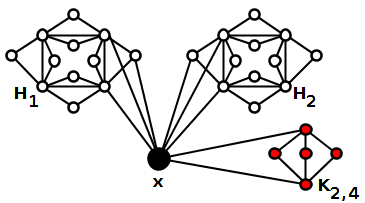
\includegraphics[width=5cm, center]{./img/grafoDobraExtremidadeObstruida2.png} &  &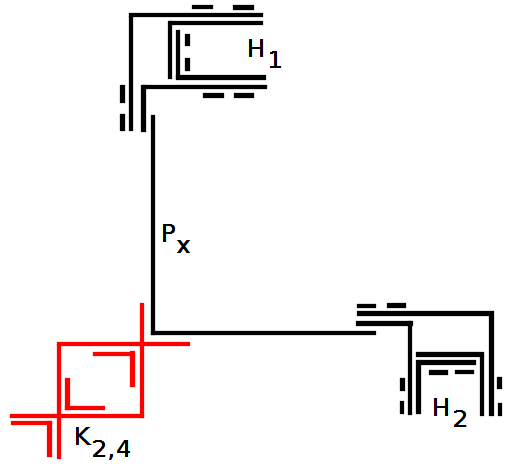
\includegraphics[width=6cm, center]{./img/extremidadeDobraObstruida5.png}  \\%[\abovecaptionskip]
    \footnotesize \centering (a) O grafo $G'$& & \footnotesize \centering (b)Uma representação $B_1$-EPG de $G'$%\\
 %   &&
  \end{tabular}
 \caption{Um exemplo de extremidade e dobra obstruída.} \label{fig:extremidadeDobraObstruida}
\end{figure}
\end{proof}




\begin{definition}
Dizemos que um segmento $s$ está \emph{internamente contido} em um caminho $P_x$ se $s$ está contido em $P_x$, e ele não intersecta uma aresta relevante de  $P_x$. 
\end{definition}

% \begin{fac}
% In a single bend representation of a graph, if a path $p(y)$ has an obstructed bend and obstructed extremities, and some path $p(x)$ intersects $p(y)$, but does not intersect paths that obstruct the extremities and the bend edges of $p(y)$, then the intersection between $p(x)$ and $p(y)$ isinternamente contida into $p(y)$. 
% \end{fac}


\begin{lema}\label{lem:volta}
Se um grafo $G_F$, construído de acordo com a definição  Definição~\ref{sec:reducao}, admite uma representação $B_1$-EPG-Helly, então a CNF-fórmula $F$ associada é uma instância-sim de {\sc Positive (1 in 3)-3sat}.
\end{lema}

% \setcounter{prove}{3}
\begin{proof}
Suponha que $G_F$ possui uma representação $B_1$-EPG-Helly, $R_{G_F}$. A partir de $R_{G_F}$ construiremos uma atribuição que satisfaz $F$. 

Primeiro, note que em toda representação de dobra simples de um $K_{2,4}$, o caminho de cada vértice do maior conjunto estável, em particular $P_{T}$ (em $R_{G_F}$), possui dobras contidas em uma torta falsa (ver Fato~\ref{fact:k24facts}). 


O vértice  $T$ é adjacente aos vértices de um triângulo de  $G_{B1}$ e $G_{B2}$. Como o $K_{2,4}$ está posicionado na dobra de  $P_{T}$, então em $R_{G_F}$ a representação de $G_{B1}$ e $G_{B2}$ devem ser posicionadas nas extremidades de $P_{T}$, ver Lema~\ref{lem:obstrucao}.   


Sem perda de generalidade, considere que $P_{V} \cap P_{T}$ é um segmento horizontal em $R_{G_F}$.

Podemos notar em $R_{G_F}$ que: o número de caminhos $P_{d}$ com segmento internamente contido em  $P_{V}$ é exatamente o número de cláusulas em $F$; a intersecção entre cada  $P_{a}, P_{e}, P_{h}$ no  dispositivo cláusula e cada caminho $P_{v_j}$ indica as variáveis que compõem a cláusula. Assim, podemos atribuir para cada variável $ x_{j}$ o valor \textit{True} se a aresta intersectante entre $P_{v_j}$ e $P_{T}$ é horizontal, e \textit{False} caso contrário. 


No Lema~\ref{lem:2vertical2horizontal} foi mostrado que qualquer representação minimal $B_1$-EPG de um dispositivo cláusula possui dois caminhos em $\{P_{a}, P_{d}, P_{e}, P_{h}\}$ com direção vertical e outros dois caminhos possuem direção horizonal. Além disso $P_{d}$ intersecta $P_{V}$, segue-se que em uma representação de dobra simples de  $G_F$ devemos conectar dois desses caminhos de forma a representar uma atribuição $False$, e exatamente um representará uma atribuição $True$. Assim, mostramos que a partir de $R_{G_F}$ podemos obter uma atribuição para $F$ tal que toda cláusula possui exatamente uma variável com valor $True$.
 \end{proof}


Note que uma representação $B_1$-EPG é  Helly se e somente se cada clique é representada por uma  clique-aresta (e não por uma  clique-garra). Mais detalhes sobre clique-aresta e clique-garra podem ser encontrados em~\cite{golumbic2009}. Assim, uma maneira alternativa para checar que uma representação é Helly seria notar que todas as cliques estão representadas como cliques-aresta.

\smallskip

Alguns vértices de  $G_F$ tem representação $B_1$-EPG altamente restritiva. O vértice $T$ possui sua dobra e ambas extremidades obstruídas por seus vizinhos, subgrafos $G_{B1}$, $G_{B2}$ e o restante do grafo $K_{2,4}$. O vértice $V$ e cada  vértice-variável $v_i$ deve ter um de seus segmentos internamente contigo em  $T$, e também suas extremidades e dobra obstruídos.  Portanto, o vértice $V$ e cada 
vértice-variável possui somente um segmento cada que pode ser utilizado em uma representação EPG para fazer a adjacência deles ao dispositivo cláusula. A direção desse segmento, começando pela horizontal ou vertical, pode ser utilizado para representar uma valoração $True$ ou $False$ para as variáveis. O  dispositivo cláusula, por outro lado, é tal que exatamente duas de suas adjacências aos vértices-variável e a $V$ pode ser efetuada com uma intersecção horizontal enquanto as outras duas  devem ser realizadas com intersecção vertical. Se considerarmos a direção utilizada por  $V$ como uma atribuição verdadeira, podemos notar que exatamente uma das variáveis em cada cláusula será $True$ em qualquer possível representação de  $G_F$. Por outro lado, é razoavelmente simples obter uma representação $B_1$-EPG para $G_F$ dada uma atribuição verdadeira para a fórmula $F$.


\begin{theorem}
{\sc Reconhecimento de grafos $B_{1}$-EPG-Helly } é NP-completo.
\end{theorem}
\begin{proof}
Pelo Teorema~\ref{teo:nppertinencia} e Lemas~\ref{lem:ida} e~\ref{lem:volta}.
 \end{proof} %$\square$

Dizemos que um grafo $k$-apex é um grafo que pode ser feito planar pela remoção de $k$ vértices. Além do mais, um grafo $d$-degenerado é um grafo em que todo subgrafo possui um vértice de grau no máximo $d$. Lembrando que  {\sc Positive (1 in 3)-3SAT} permanece $NP$-completo quando o grafo de incidência da fórmula de entrada é planar~\cite{mulzer2008minimum}. Assim, o seguinte corolário é válido.

\begin{corollary}
 \label{coro:2apexAnd3degenerate}
{\sc Reconhecimento de grafos $B_{1}$-EPG-Helly} é NP-completo sobre grafos $2$-apex e $3$-degenerado.
\end{corollary}

\begin{proof}
É fácil ver que os grafos construídos de acordo com a Definição~\ref{sec:reducao} são $3$-degenerados.
Como {\sc Positive (1in3)-3SAT} permanece $NP$-completo quando o grafo de incidência da fórmula  $F$ é planar~\cite{mulzer2008minimum},  de uma instância $F$ de {\sc Planar Positive (1in3)-3SAT}, então usando uma representação planar do grafo de incidência de $F$, podemos observar que pela remoção de $V$ e $T$ de $G_F$ obtemos um grafo planar. Logo, $G_F$ é 2-apex. 
\end{proof}


Para provar que $G_F$ é 3-degenerado basta aplicar o algoritmo de reconhecimento de grafos $d$-degenerados, que consiste em repetidamente remover os vértices de grau mínimo do grafo. Note que o vértice a ser removido a cada iteração do algoritmo sempre possui grau no máximo três, e portanto $G_F$ é 3-degenerado.

%Para elucidar o Corolário~\ref{coro:2apexAnd3degenerate}, que pode não ser trivial, sugerimos o seguinte raciocínio para provar que $G_F$ é 3-degenerado: aplicar o algoritmo de reconhecimento de grafos $d$-degenerados. 
A título de exemplo apresentamos a seguir uma construção para esclarecer a segunda parte do corolário. Tomemos a fórmula $F=(x_1+x_2+x_3)\wedge(x_1+x_3+x_4)\wedge(x_1+x_2+x_4)$, que  é uma instância de {\sc Planar Positive (1in3)-3SAT} e vamos mostrar que o dispositivo específico $G_F$ gerado a partir dessa instância é um grafo 2-apex.

Primeiro, monte o grafo de incidência de $F$, chamemos ele de $I_F$. O grafo de incidência é um grafo bipartido onde uma das partições está relacionada com as cláusulas de $F$ e a outra partição está relacionada com as suas variáveis. Cada cláusula $C_i$ de $F$ é representada por um vértice $v_{c_i}$ e cada variável $x_j$ das cláusulas é representada por um vértice $v_{x_j}$. Uma aresta  $(v_{c_i}, v_{x_j})$ existe em $I_F$ se e somente se a variável $x_j$ ocorre na cláusula $C_i$. A Figura~\ref{fig:grafoIncidencia2apex} retrata uma construção do grafo de incidência $I_F$.

\begin{figure}[htb]	
\center%6.3
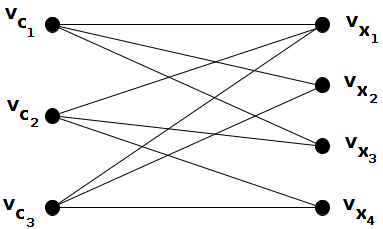
\includegraphics[width=6cm]{./img/grafoIncidencia2apex.png}
\caption{Grafo de incidência $I_F$, formato bipartição }
\label{fig:grafoIncidencia2apex}
\end{figure}

Como a fórmula $F$ que originou o grafo $I_F$ é uma instância de {\sc Planar Positive (1in3)-3SAT}, sabemos que o grafo de incidência da fórmula  $F$ é também planar~\cite{mulzer2008minimum}. A Figura~\ref{fig:grafoIncidencia2apexPlanar} retrata uma representação planar de $I_F$.


\begin{figure}[htb]	
\center%6.3
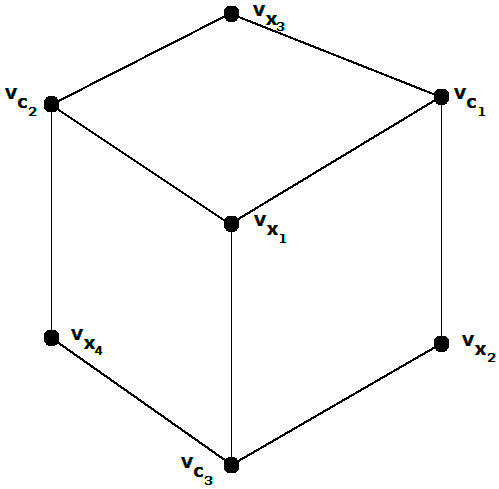
\includegraphics[width=8cm]{./img/grafoIncidencia2apexPlanar.png}
\caption{Grafo de incidência $I_F$ em uma representação planar }
\label{fig:grafoIncidencia2apexPlanar}
\end{figure}

Finalmente, podemos substituir os vértices que representavam as variáveis e cláusulas em $I_F$ pelos dispositivos variáveis e cláusulas correspondentes. Os vértices $V$ e $T$ são removidos. Como cada dispositivo variável, dispositivo cláusula e dispositivo base individualmente era planar, então algo não planar pode ter surgido somente da intersecção que foi feita entre eles. Como $I_F$ garante que existe um arranjo planar entre as intersecções dos dispositivos variável e dispositivos cláusula, então quando removemos $V$ e $T$, tudo o que sobra do grafo é planar, ver Figura~\ref{fig:grafoIncidenciaCompleto}. Logo $G_F$ é 2-apex.


\begin{figure}[htb]	
\center%6.3
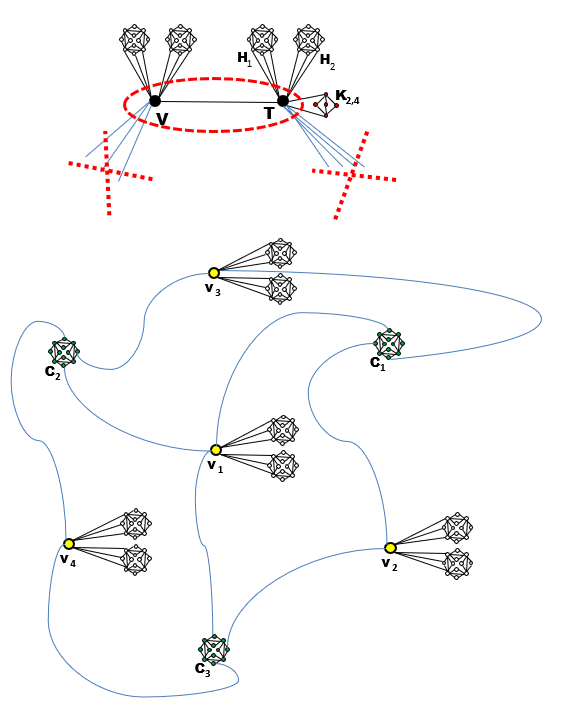
\includegraphics[width=10cm]{./img/grafoIncidenciaCompleto.png}
\caption{Grafo planar $G_F$, obtido a partir de $I_F$, a menos dos vértices $V$ e $T$ }
\label{fig:grafoIncidenciaCompleto}
\end{figure}
  \chapter{O número de Helly e o número de Helly forte para grafos $B_k$-EPG e $B_k$-VPG}


\begin{flushright}
\begin{minipage}[t][0cm][b]{0.47\textwidth}
\emph{
%A Matemática é o alfabeto com o qual Deus escreveu o Universo.
Falta algo para completar esta demonstração, mas não tenho tempo.}
\end{minipage}

\rule[0cm]{7cm}{0.03cm}%{largura}{espessura}

Évariste Galois
\end{flushright}




O estudo de grafos EPG foi introduzido por  Golumbic, Lypshteyn e Stern (2009) e consiste dos grafos de intersecção de conjuntos de caminhos sobre uma grade ortogonal, cujas intersecções são tomadas considerando as arestas dos caminhos. Se as intersecções dos caminhos consideram os vértices e não as arestas, a classe de grafos resultante é chamada de grafos VPG. Tal classe foi introduzida em 2011 \cite{asinowski2011string} e \cite{asinowski2012}. Nesse capítulo estudaremos dois parâmetros em ambas classes de grafos EPG e VPG. Os parâmetros que serão estudados são nomeadamente o número de Helly e o número de Helly forte.

\section{Discussão Inicial}

Seja  $\cal {F}$ uma família de conjuntos de algum conjunto universal $U$, e $h$ um número inteiro tal que $h\geq 1$. Podemos dizer que $\cal{F}$ é $h$-{\it intersectante} quando todos  $h$ subconjuntos de $\cal {F}$ intersectam-se. Chamamos de {\it core} de $\cal {F}$ a intersecção de todos conjuntos de $\cal {F}$, e denotamos por $core(\cal F)$. 

A família $\cal{F}$ é $h$-{\it Helly} quando toda subfamília $h$-intersectante $\cal{F'}$ satisfaz $core(\cal{F'}) \neq \emptyset$, ver mais em \cite{duchet1978propriete}. Por outro lado, se para toda subfamília $\cal{F'}$ de $\cal{F}$, existem $h$ subconjuntos cujo core é igual ao core de  $\cal {F'}$, então $\cal {F}$ é dito ser  $h$-{\it Helly} {\it forte}. Claramente, se $\cal {F}$ é $h$-Helly então ele também é $h'$-Helly, para $h' \geq h$. Similarmente, se ${\cal F}$ é $h$-Helly forte então ele também é $h'$-Helly forte, para $h' \geq h$. 

Finalmente, o   {\it número de Helly} da família  $\cal{F}$ é o menor inteiro $h$, tal que $\cal{F}$ é  $h$-Helly. Similarmente, o {\it número de Helly forte} de  $\cal{F}$ é o menor $h$, para o qual  $\cal{F}$ é  $h$-Helly forte. Também segue que o número de Helly forte de $\cal{F}$ é no mínimo igual ao seu número de Helly.


Uma  {\it classe} $\cal {C}$ de famílias $\cal {F}$  de subconjuntos de algum conjunto universal $U$ é uma  subcoleção das famílias $\cal {F}$ de $U$. Dizemos que  $\cal C$ é uma {\it classe hereditária}, quando ela é fechada sob inclusão, i.e. se um grafo $G$ pertence a uma classe $C$ então todo subgrafo induzido de $G$ também pertence a $C$. O {\it número de Helly}  de uma classe  $\cal{C}$ de famílias $\cal{F}$ de subconjuntos é o maior número de Helly entre todas as famílias de $\cal {F}$. Similarmente, o {\it número de Helly forte} de uma classe  $\cal {C}$ é o maior número de Helly forte das famílias de $\cal {C}$.

Se $\cal F$ é uma família de subconjuntos e $\cal C$ uma classe de famílias, denotamos por $H(\cal F)$ e por 
$H(\cal C)$,  o número de  Helly de $\cal F$ e $\cal C$, respectivamente, enquanto  $sH({\cal F})$ e $sH({\cal C})$  representam os números de  Helly forte de $\cal F$ e $\cal C$.


Nesse capítulo, nos preocupamos com famílias de subconjuntos $\cal{F}$ de caminhos de arestas e vértices em uma grade. No primeiro contexto, consideramos que cada caminho $P_i$  consiste de uma sequência de arestas consecutivas na grade ortogonal, que forma o caminho, e chamaremos essas de   {\it representações EPG}. Dessa forma, segue que dois caminhos intersectam-se se e somente se eles contém no mínimo uma aresta da grade em comum. Aos grafos que  correspondem às representações EPG denotaremos por {\it grafos EPG}. 
No segundo contexto, um caminho é visto como uma sequência de vértices consecutivos, e dois caminhos intersectam-se se eles contém um vértice comum. Analogamente aos anteriores esses são chamados de {\it representações VPG} e {\it grafos VPG}. 

Cada aresta possui uma direção associada na grade, a qual pode ser horizontal ou vertical. Uma  {\it dobra} no caminho é um par de arestas consecutivas que possuem direções distintas.  Um {\it segmento} de um caminho é uma sequência de arestas consecutivas do caminho, sem dobras. Dizemos que o caminho $P_i$ é um  $B_k$-{\it path} se ele contém $k$ dobras. Dizemos que $\cal {F}$ é uma família de $B_k$-caminhos, ou simplesmente  uma $B_k$-família, se cada caminho de $\cal {F}$ contém no máximo $k$ dobras. 

 Nesse capítulo, resolvemos completamente o problema de determinar ambos o número de Helly e o número de Helly forte, para ambos contextos de grafos $B_k$-EPG e $B_k$-VPG. Determinamos o número de Helly em grafos $B_k$-EPG e $B_k$-VPG, para cada valor de $k$.

Para grafos EPG, o número de Helly de $B_0$-families é bem conhecido e é igual a 2, uma vez que  grafos $B_0$-EPG coincidem com grafos de intervalo. Também é simples concluir que o número de Helly forte dos grafos $B_0$-EPG é também igual a 2. Para $k = 1$,   provamos que ambos o número de Helly e número de Helly forte da classe de $B_1$-families são iguais a 3. Para a classe de  $B_2$-families, provamos que esses dois parâmetros são iguais a 4. Além disso o número de Helly e número de Helly forte para $B_3$-families é igual a 8, e finalmente esses parâmetros são ilimitados para  $k \geq 4$. 
Quanto aos grafos VPG, é simples concluir que o número de Helly de grafos $B_0$-VPG é igual a 2, e provamos que grafos $B_1$-VPG possuem número de Helly  4, grafos $B_2$-VPG possuem número de Helly  6, grafos $B_3$-VPG possuem número de Helly 12, enquanto o número de Helly para grafos $B_4$-VPG novamente é ilimitado.

Finalmente, o número de Helly forte é igual ao número de Helly nos grafos  $B_k$-EPG, para cada $k$. O mesmo vale para grafos $B_k$-VPG.

Com relação aos resultados existentes, 
Golumbic, Lipshteyn  e Stern \cite{golumbic2009} já tem mostrado que o número de Helly forte para grafos $B_1$-EPG é igual a 3, e para grafos $B_1$-VPG é igual a  4. Empregando técnicas de prova diferentes das utilizadas neste trabalho. Veja  \cite{golumbic2019edge}, Teorema 11.13, abaixo:
\begin{theorem}\label{thm:golumbic2019edge}{\cite{golumbic2019edge}}
Seja $P$ uma coleção de caminhos de dobra simples sobre uma grade. Se cada 2 caminhos em  $P$ compartilham no mínimo uma aresta da grade, então $P$ possui número de Helly forte igual a 3. Caso contrário, $P$ possui número de Helly forte igual a 4. 
\end{theorem}
Nenhum outro resultado relacionado ao número de Helly forte, ou resultados relacionados ao número de Helly de grafos $B_k$-EPG foi notado ter sido reportado na literatura levantada. Quanto a outras classes, Golumbic e Jamison  tem determinado o número de Helly forte dos caminhos de intersecção de arestas sobre uma árvore em~\cite{golumbic1985}. Finalmente, Asinowski, Cohen, Golumbic, Limouzy, Lipshteyn e Stern tem reportado que o número de Helly forte de grafos $B_0$-VPG é igual a 2 \cite{asinowski2011string}.  
Alguns resultados relacionados estão listados a seguir. Decidir se um dado hipergrafo é  $k$-Helly pode ser feito em tempo polinomial para um  $k$ fixo,  empregando a caracterização proposta por Berge e Duchet \cite{bergeDuchet1975}. Para algum $k$ arbitrário, o problema é  \cal{co-NP}-completo \cite{dourado2009}. Para ver mais problemas correspondendo à propriedade $k$-Helly forte e exemplos sugerimos a leitura de~\cite{dourado2008strong,dourado2009}.

Este capítulo está organizado como listado a seguir. A seção~\ref{sec:preliminares4}, contém algumas proposições preliminares e notações adicionais utilizadas neste escrito. A seção~\ref{sec:Helly-number}  descreve os resultados para o número de Helly de grafos $B_k$-EPG, enquanto a seção~\ref{sec:helly-vpg} contém resultados desse parâmetro para grafos $B_k$-VPG. O número de Helly forte é considerado na seção~\ref{sec:helly-forte}. Considerações finais são efetuadas na seção~\ref{sec:finalRemarks4}.

\section{Preliminares}\label{sec:preliminares4}

O seguinte teorema caracteriza famílias de subconjuntos $h$-Helly.


\begin{theorem}\label{thm:BD}(\cite{bergeDuchet1975}):
Uma família $\cal{F}$ de subconjuntos do conjunto universal  $U$ é $h$-Helly se e somente se para todo subconjunto   $U' \subseteq U$, $|U'|= h+1$,  a subfamília  $\cal{F'}$ de $\cal{F}$,  formada pelos subconjuntos contendo no mínimo  $h$ dos $h+1$ elementos de $U'$, tem um core não vazio. 
\end{theorem}

O próximo teorema é central para os nossos resultados.

\begin{theorem}\label{thm:minimal}Seja ${\cal C}$ uma classe hereditária de famílias ${\cal F}$ de subconjuntos do conjunto universal $U$, cujo número de Helly $H({\cal C})$ é igual a $h$. Então, existe uma família ${\cal F'} \in {\cal C}$ com exatamente $h$ subconjuntos, satisfazendo as seguintes condições: 

Para cada subconjunto  $P_i \in \cal {F'}$, existe exatamente um elemento distinto $u_i \in U$, tal que \\
$$u_i \not \in P_i,$$ 
mas $u_i$ está contido em todos subconjuntos 
$$P_j \in {\cal F'} \setminus P_i.$$
\end{theorem}
 

Proof: 
Seja ${\cal C}$ uma classe de famílias  ${\cal F}$ de subconjuntos $P$, cada subconjunto formado pelos elementos  $u \in U$, tal que o número de Helly $H({\cal C})$  é igual a $h$. Então cada família   ${\cal F} \in {\cal C}$ satisfaz $H({\cal F}) \leq h$. Considere uma família ${\cal F'} \in {\cal C}$  cujo número de Helly é  exatamente $h$, e contendo exatamente $h$ subconjuntos. Essa família deve existir uma vez que  ${\cal C}$ é uma classe hereditária. Além disso $H({\cal F'}) = h$, $\cal F'$ é $h$-intersectante, e portanto $(h-1)$-intersectante. Ademais, ${\cal F'}$ não é $(h-1)$-Helly. Aplicando o   Teorema~\ref{thm:BD}, podemos concluir que existem   $h$ elementos $U' = \{u_1, \ldots, u_h\} \subset U$, tal que cada conjunto de ${\cal F'}$ contem no mínimo $h-1$ elementos de $U'$. Uma vez que $H({\cal F'}) > h-1$, $core({\cal F'}) = \emptyset$ e além disso não existe elemento comum entre os conjuntos de $\cal F'$. Em particular, uma vez que cada conjunto $P_i \in {\cal F'}$ contem no mínimo  $h-1$ elementos de $U'$, e $core(\cal F') = \emptyset$, podemos escolher   $h$ subconjuntos $P_i$, em que cada um deles deixa de possuir um elemento distinto  $u_i \in U'$. Então para cada subconjunto  $P_i \in \cal F$, existe algum elemento $u_i \not \in P_i$, mas $u_i \in P_j$, para todos $P_j \in \cal F'$, $j \neq i$. \qed

Seja $\cal{ F'}$ como descrito no teorema anterior. É simples concluir que ao remover qualquer subconjunto de $\cal {F'}$ este torna-se $(h-1)$-Helly.  Todavia podemos chamar $\cal {F'}$ de uma {\it família minimal não}-$(h-1)$-{\it Helly}. Além do mais, o elemento $u_i \not \in P_i$, contido em todos os subconjuntos $P_j \in {\cal{F'}} \setminus P_i$, exceto $P_i$, é o {\it $h$-não-representativo} de $P_i$.  

Empregaremos as famílias de subconjuntos minimais citadas anteriormente, aplicadas à $B_k$-caminhos em uma grade. Note que $B_k$-caminhos em uma grade formam uma classe hereditária.

\section{O Número de Helly de Grafos $B_k$-EPG}\label{sec:Helly-number}

Nessa seção determinaremos o número de Helly das classes de grafos $B_1$-EPG, $B_2$-EPG e $B_3$-EPG, e mostraremos que para os grafos $B_k$-EPG, $k \geq 4$, o número de Helly é ilimitado. Provaremos os seguintes resultados.

\begin{theorem}\label{thm:Helly-EPG}
O número de Helly de grafos $B_k$-EPG satisfaz:
\begin{enumerate}[nosep,label=\emph{(\roman*)}]
\item  $H(B_1$-EPG) = 3 
\item $H(B_2$-EPG)  = 4 
\item $H(B_3$-EPG)  = 8 
\item $H(B_k$-EPG) é ilimitado, para 
$k \geq 4$.
\end{enumerate}

\end{theorem}

A prova consiste em determinar limites inferiores e limites superiores justos, como mostrado nas próximas subseções.

\subsection{Limites Inferiores}

Primeiro, descreveremos limites inferiores para o parâmetro número de Helly, como função do número de dobras $k$.

\begin{lema}\label{claim:lower-Bk-EPG} 
Os seguintes são limites inferiores para os grafos  $B_k$-EPG.
\begin{enumerate}[nosep,label=\emph{(\roman*)}]
\item   $H(B_1$-$EPG) \geq 3$ 
\item $H(B_2$-$EPG) \geq 4$ 
\item $H(B_3$-$EPG) \geq 8$ 
\item $H(B_k$-$EPG )$ é ilimitado para  $k \geq 4$.
\end{enumerate}
\end{lema}

\proof:

Para cada valor de  $k$, exibiremos uma $B_k$-família de caminhos em arestas na grade, tendo o número de dobras requerido, e cujo número de Helly é no mínimo o valor correspondente declarado. Nos referimos ao par de coordenadas dos pontos da grade (arestas da grade), de forma a descrever os caminhos.

\begin{figure}[!h]
\begin{center}
% \begin{tikzpicture}[line cap=round,line join=round,>=triangle 45,x=3.7mm,y=3.7mm]
% \draw [color=cqcqcq,, xstep=0.37cm,ystep=0.37cm] (-7,-1.4) grid (22.16,6.8);
% \clip(-5.7,-2.5) rectangle (25,9.6);
% \draw (-5,-1.3) node[anchor=north west] {(a)};
% \draw (2.5,-1.3) node[anchor=north west] {(b)};
% \draw (14.5,-1.3) node[anchor=north west] {(c)};
% \draw [line width=2pt] (4,0)-- (4,2)-- (6,2)-- (6,0);
% \draw [line width=2pt] (3,2)-- (1,2)-- (1,0)-- (3,0);
% %\draw (-0.3,3.7) node[anchor=north west] {0};
% %\draw (-0.3,5.1) node[anchor=north west] {1};
% %\draw (-0.3,6.1) node[anchor=north west] {2};
% \draw [line width=2pt] (1,5)-- (3,5)-- (3,3)-- (1,3);
% \draw [line width=2pt] (4,5)-- (4,3)-- (6,3)-- (6,5);
% %\draw (8.7,0.7) node[anchor=north west] {0};
% %\draw (8.7,2.1) node[anchor=north west] {1};
% %\draw (8.7,3.1) node[anchor=north west] {2};
% %\draw (8.7,3.7) node[anchor=north west] {0};
% %\draw (8.7,5.1) node[anchor=north west] {1};
% %\draw (8.7,6.1) node[anchor=north west] {2};
% \draw [line width=2pt] (10,5)-- (12,5)-- (12,3)-- (10,3)-- (10,4);
% \draw [line width=2pt] (14,5)-- (13,5)-- (13,3)-- (15,3)-- (15,5);
% \draw [line width=2pt] (19,3)-- (19,5)-- (21,5)-- (21,3)-- (20,3);
% \draw [line width=2pt] (18,4)-- (18,5)-- (16,5)-- (16,3)-- (18,3);
% \draw [line width=2pt] (10,1)-- (10,2)-- (12,2)-- (12,0)-- (10,0);
% \draw [line width=2pt] (13,2)-- (13,0)-- (15,0)-- (15,2)-- (14,2);
% \draw [line width=2pt] (20,0)-- (19,0)-- (19,2)-- (21,2)-- (21,0);
% \draw [line width=2pt] (18,2)-- (16,2)-- (16,0)-- (18,0)-- (18,1);
% \draw [line width=2pt] (-6,2.25)-- (-4.25,2.25)-- (-4.25,4);
% \draw [line width=2pt] (-3.75,4)-- (-3.75,2.25)-- (-2,2.25);
% \draw [line width=2pt] (-6,1.75)-- (-2,1.75);
% \end{tikzpicture}
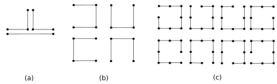
\includegraphics[width=12cm]{./img/b1epgSub.pdf}
\end{center}
\caption{Subfamílias Minimais não-Helly para $B_1$, $B_2$ e $B_3$ -families.}
\label{fig:b1b2b3families}
\end{figure}

Para $k=1$, seja $\cal{F}$ uma família de três caminhos de 1-dobra que são mutuamente intersectantes mas que não possuem aresta em comum, como ilustrado na Figura~\ref{fig:b1b2b3families}$(a)$. 
%For $k=1$, let $\cal{F}$ be the família %of three 1-dobra caminhos, $P_1: (0,0),(0,1),(1,1)$; $P_2: (1,1), (1,0),(0.2)$; and $P_3: (0,0),(0,2)$.  See Figure   $1a$. 
Então $\cal{F}$ é uma família de três caminhos  2-intersectante e $B_1$-EPG, tendo um core vazio. Portanto, $H(B_1$-EPG$) \geq 3$. 
Além disso, pela remoção de qualquer dos caminhos o core de $\cal{F}$ torna-se não-vazio. Todavia $\cal{F}$ é uma família de caminhos minimal não 2-Helly.

Seja $S$ o 4-ciclo, formado pelos 4 segmentos de pares de arestas, com dobras nos seguintes pontos da grade $(0,0),(0,2),(2,2),(2,0)$, respectivamente.
 Para $k= 2$,  considere $\cal{F}$ ser a família de quarto caminhos de 2-dobras formada quando removemos exatamente um par de arestas que formam os segmentos de cada lado do 4-ciclo, como ilustrado na  Figura~\ref{fig:b1b2b3families}$ (b)$.
Segue que $\cal{F}$ é 3-intersectante e seus caminhos não possuem nenhuma aresta comum. Consequentemente $H(B_2$-EPG)$ \geq 4$.

Para $k=3$, considere a família $\cal{F}$ de oito caminhos de  3-dobras, respectivamente, que podem ser obtidos de $S$. O 4-ciclo $S$ contem exatamente  8 arestas da grade. A  família $\cal{F}$ consiste de oito caminhos $P_i$, $1 \leq i \leq 8$, obtidos pela remoção de $S$, exatamente uma dessas oito arestas distintas, como ilustrado na Figura~\ref{fig:b1b2b3families} $ (c)$. Consequentemente, $\cal{F}$ é 7-intersectante, mas $core({\cal{F}}) = \emptyset$. Portanto, $H(B_3$-EPG)$\geq 8$.

Finalmente, para $k = 4$, seja $\cal{F}$ a família de $n$ $B_4$-caminhos $P_i$, descrita como segue:

\begin{itemize}
    \item $P_1$ é formado pelos segmentos: \\ $(0,0),(0,1),(1,1),(1,0),(n,0)$; 

     \item para $2 \leq i \leq n-1$, $P_i$ contem os segmentos: \\
     $(0,0),(0,i-1),(i-1,1),(i,1),(i,0),(n,0)$;
     
     \item  $P_n$ é formado pelos seguintes segmentos: \\ $(0,0),(n-1,0),(n-1,1),(n-1,0).$
     
\end{itemize}     

Observe que $\cal{F}$ é $(n-1)$-intersectante, enquanto $core({\cal{F}})=\emptyset$. Veja a Figura~\ref{fig:figurab4}. Dessa forma $H(B_4$-EPG) é ilimitado. Claramente o mesmo vale para $k >4$. \qed  



\begin{figure}[!h]
\begin{center}
% \begin{tikzpicture}[line cap=round,line join=round,>=triangle 45,x=3.7mm,y=3.7mm]
% \draw [color=cqcqcq,, xstep=0.74cm,ystep=0.74cm] (-7,-1.0) grid (22.8,14.8);
% \clip(-6.7,-1.8) rectangle (27,14.6);
% \draw [line width=2pt] (-6,0)-- (-6,2)-- (-4,2)-- (-4,0)-- (22,0);

% \draw [line width=2pt] (-6,4)-- (-4,4)-- (-4,6)-- (-2,6)-- (-2,4)-- (22,4);

% %\draw [line width=2pt] (-6,6)-- (-2,6)-- (-2,8)-- (0,8)-- (-0,6)-- (22,6);

% \draw [line width=2pt] (-6,8)-- (10,8)-- (10,10)-- (12,10)-- (12,8)-- (22,8);

% \draw [line width=2pt] (-6,12)-- (20,12)-- (20,14)-- (22,14)-- (22,12);


% \draw (6.5,6.5) node[anchor=north west] {.};
% \draw (6.5,7) node[anchor=north west] {.};
% \draw (6.5,7.5) node[anchor=north west] {.};

% \draw (6.5,10.5) node[anchor=north west] {.};
% \draw (6.5,11) node[anchor=north west] {.};
% \draw (6.5,11.5) node[anchor=north west] {.};

% \draw (-5.65,0.4) node[anchor=north west] {1};
% \draw (-3.65,3.4) node[anchor=north west] {2};

% %\draw (-1.65,6.4) node[anchor=north west] {3};

% \draw (10.35,8.4) node[anchor=north west] {i};

% \draw (20.35,12.4) node[anchor=north west] {n};

% \end{tikzpicture}
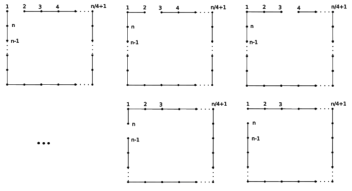
\includegraphics[width=12.5cm]{./img/b4epg.pdf}
\end{center}
\caption{$B_4$ possui número de Helly ilimitado.}\label{fig:figurab4}
\end{figure}

A seguir, nos preocupamos em encontrar limites superiores para grafos $H(B_k$-EPG).

\subsection{Limites Superiores}\label{subsec-upper}

De forma a obter um limite superior justo para o número de Helly, em termos do número de dobras, introduzimos abaixo mais algumas notações e lemas.

Dizemos que um conjunto de arestas da grade é {\it co-linear} se todas arestas do conjunto pertencem a uma mesma linha da grade, horizontal ou vertical. O conjunto de arestas é chamado {\it paralelo} se todas as suas arestas estiverem sobre linhas paralelas da grade mas nenhuma delas for co-linear.


\begin{lemma}
\label{lemma:3colin}
Seja $\cal {F}$ uma família minimal não-$(h-1)$-Helly de caminhos sobre uma grade contendo três arestas co-lineares não representativas. Então $\cal{F}$ deve conter caminhos com no mínimo quatro dobras.
\end{lemma}

\proof
Seja  $u_i$ a aresta do meio entre as três arestas  co-lineares não representativas. Ela corresponde ao caminho $P_i$ de $\cal {F'}$, não contendo $u_i$.
 Então $P_i$ deve passar pelas outras duas arestas mas ele não deve incluir a aresta do meio. Portanto, o caminho $P_i$ deve sair da linha comum da grade, contendo essas três arestas representativas, e retornar à mesma linha, assim requerendo no mínimo quatro dobras.
\qed


\begin{lemma}
\label{lemma:3par}
Seja $\cal{F}$ uma família minimal não-$(h-1)$-Helly de caminhos sobre uma grade, contendo três arestas paralelas, e tendo número de Helly $H(\cal{F})$   $\geq 4$. Então $\cal{F}$ deve conter caminhos com no mínimo quatro dobras. 
\end{lemma}

\proof
Uma vez que $H(\cal{F}) $ $\geq 4$ e $\cal{F}$ é uma $(h-1)$-família minimal, segue que $\cal{F}$ deve conter no mínimo quatro caminhos, $P_1,P_2,P_3,P_4$. Sem perda de generalidade, sejam $u_1,u_2,u_3$ as arestas não-representativas dos caminhos $P_1,P_2,P_3$ que são paralelas. Então $P_4$ deve passar por todas três arestas paralelas não-representativas $u_1,u_2,u_3$, assim requerendo no mínimo quatro dobras. 
\qed


\begin{lemma} \label{lemma:Lwit}
Seja $\cal{F}$ uma família minimal não-$(h-1)$-Helly de caminhos sobre uma grade com  número de Helly $H({\cal F}) \geq 4$. Se  ${\cal F}$ contem três arestas  não-representativas que se encontram sobre um mesmo $B_1$-caminho  $P_1$ de $\cal{F}$, então $\cal {F}$ deve possuir algum caminho com no mínimo três dobras. \end{lemma}

\proof
Visto que $\cal{F}$ é uma  $(h-1)$-família minimal tendo  número de Helly $\geq 4$, ela contem no mínimo quatro caminhos. Sem perda de generalidade, sejam  $u_1, u_2, u_3$ as três arestas não-representativas contidas em $P_4$ e tal que  $u_2$ encontra-se entre $u_1$ e $u_3$ em $P_4$. Então o caminho $P_2$ deve conter $u_1$ e $u_3$, mas evite $u_2$, assim requerendo no mínimo três dobras.  
\qed

A seguir são apresentados os limites superiores justos para os números de Helly de $B_k$-caminhos em arestas, para $k = 1,2,3$.

\begin{lema}\label{claim:upper-B1}
$H(B_1$-$EPG) \leq 3.$
\end{lema}
 
\proof
Assuma por contradição que o número de Helly de famílias de caminhos $B_1$-EPG é $h > 3$. Nesse caso, considere uma família minimal não-$(h-1)$-Helly de $\cal F$ de $B_1$-caminhos. Então $\cal F$ contem no mínimo  $h$ caminhos.  
Qualquer caminho $P_1 \in \cal{F}$ deve conter $h-1$ arestas não-representativas  correspondendo aos $h-1$ distintos caminhos de $\cal F$, diferentes de $P_i$. Uma vez que $h-1 \geq 3$, $P_1$  contem no mínimo três arestas  distintas não-representativas $u_2, u_3, u_4 \in P_1$, com $u_3$ encontrando-se entre $u_2$ e $u_4$ no caminho.  Se $P_1$ não possui dobras, $u_2,u_3,u_4$ são co-lineares. Pelo Lemma~\ref{lemma:3colin},  o caminho $P_3 \in \cal{F}$ deve conter no mínimo quatro dobras. Se $P_1$ possui exatamente uma dobra, segue do Lemma~\ref{lemma:Lwit} que $P_3$ possui três dobras. Em qualquer situação, uma contradição surge, implicando que $H({\cal F}) \leq 3$.
\qed

\begin{lema}\label{claim:upper-B2}
$H(B_2$-EPG$) \leq 4.$
\end{lema}

\proof
Assume by contradiction that the número de Helly of  $B_2$-EPG families of caminhos is $h > 4$. In this case, consider a minimal não-$(h-1)$-Helly família $\cal F$ of $B_2$-EPG caminhos. The família  $\cal F$ must contain at least $h \geq 5$ distinct caminhos, each of them corresponding to a distinct não-representativo  edge. Choose arbitrarily 5 of these não-representativo edges.

By Lemmas ~\ref{lemma:3colin} and ~\ref{lemma:3par} any three of these chosen edges can  neither be co-linear nor parallel. Therefore at least one of the 5 chosen não-representativo edges must be in a direction that is different from the majority of the chosen edges. Call the direction of this edge vertical, and the direction of the majority of the chosen edges horizontal. Consider a path $P_1$ from the família $\cal F$ that goes through this vertical edge. 
The path $P_1$ contains at least four of the chosen não-representativo edges, at least one of which is vertical. Since $P_1$ has at most 2 dobras then it must have at most three segments. Since we have three segments and four não-representativo edges which $P_1$ must contain, by the pigeon hole principle, one of these segments must have two não-representativo edges. If this pair of edges are in a horizontal segment of $P_1$, then such  pair of edges, along with the vertical edge are in two consecutive path segments, forming a $B_1$-subpath in $\cal F$. Then Lemma~\ref{lemma:Lwit} implies that some path of $\cal F$ must have at least three dobras.   Otherwise, the two edges are vertical. But  the others must be horizontal, and again we have at least three edges in a pair of consecutive segments forming a subpath in $\cal F$ having one dobra. Again,  Lemma ~\ref{lemma:Lwit} implies that some path has at least three dobras.
\qed

\begin{lema}\label{claim:upper-B3}
$H(B_3$-EPG$) \leq 8.$
\end{lema}

\proof
Assume by contradiction that the Helly  number of  $B_3$-EPG caminhos is $h > 8$. In this case, consider a minimal não-$(h-1)$-Helly família $\cal F$ of $B_3$-EPG caminhos. Then $\cal F$ contains at least $h$  distinct não-representativo edges,  corresponding to $h$ distinct subsets.  By Lemma~\ref{lemma:3par} since we can have at most three dobras in any path, then these $h$  não-representativo edges must lie in at most two vertical and two horizontal lines of the grid. Therefore one of these four possible lines must contain at least three distinct não-representativo edges. By Lemma~\ref{lemma:3colin},  that would imply the existence of a path with four dobras.\qed

This completes the proof of Theorem \ref{thm:Helly-EPG}. 


\section{Número de Helly of $B_k$-VPG Graphs}\label{sec:helly-vpg}

In this section, we determine the número de Helly of $B_k$-VPG graphs. We prove the following results.
\begin{theorem}\label{thm:Bk-VPG}
The número de Hellys for $B_k$-VPG graphs satisfy:
\begin{enumerate}
\item $H(B_1$-VPG) = 4
\item $H(B_2$-VPG) = 6
\item $H(B_3$-VPG) = 12
\item $H(B_4$-VPG) is unbounded.
\end{enumerate}
\end{theorem}

Again, we prove the theorem by showing tight lower and upper bounds.

\subsection{Lower Bounds}

First, we describe lower bounds.

Figure \ref{VPG:lower-B1} shows a set of 4 $B_1$-caminhos of a graph $G$, in a $2 \times 2$ grid, such that each path covers 3  vertices of $G$, and avoids exactly one of the  vertices. 

\begin{figure}[!h]
    \centering
    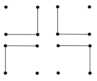
\includegraphics[width=3cm]{./img/lower-bound-B1-VPG.pdf}
    \caption{Lower bound for $B_1$-VPG graphs}
    \label{VPG:lower-B1}
\end{figure}

Figure \ref{VPG:lower-B2} shows a set of 6 $B_2$-caminhos of a graph $G$, in a $2 \times 3$ grid, such that each path covers 5  vertices of $G$, and avoids exactly one. 


\begin{figure}[!h]
    \centering
    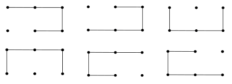
\includegraphics[width=8cm]{./img/lower-bound-B2-VPG.pdf}
    \caption{Lower bound for $B_2$-$VPG$ graphs}
    \label{VPG:lower-B2}
\end{figure}


Figure \ref{VPG:lower-B3} shows 12 $B_3$-caminhos of a graph $G$, in a grid, of perimeter 12, such that each path covers 11  vertices of $G$,  avoiding one of them. 

\begin{figure}[!h]
    \centering
    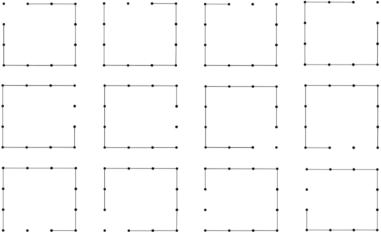
\includegraphics[width=12cm]{./img/lower-bound-B3-VPG.pdf}
    \caption{Lower bound for $B_3$-VPG graphs}
    \label{VPG:lower-B3}
\end{figure}

Figure \ref{VPG:lower-B4} shows a set of $n$ $B_4$-caminhos of a $n$-vertex graph $G$, in a grid having perimeter $n$,  such that each path covers $n-1$  vertices of $G$, avoiding one of them. 

\begin{figure}[!h]
    \centering
    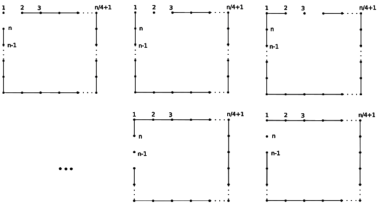
\includegraphics[width=12cm]{./img/lower-bound-B4-VPG.pdf}
    \caption{Lower bound for $B_4$-VPG graphs}
    \label{VPG:lower-B4}
\end{figure}

Applying Theorem \ref{thm:minimal}, we can then conclude that the number of vertices of each of the above described graphs are lower bounds for the corresponding class. Then, we can claim the following bounds.

\begin{lema}\label{claim:VPG-lower}
The following are lower bounds for $H(B_k$-VPG) graphs.
\begin{enumerate}
\item $H(B_1$-VPG) $\geq 4$
\item $H(B_2$-VPG) $\geq 6$
\item $H(B_3$-VPG) $\geq 12$
\item $H(B_4$-VPG) is unbounded.
\end{enumerate}
\end{lema}

\subsection{Upper Bounds}

Next, we provide upper bounds for the número de Helly of $B_k$-VPG graphs. The following lemmas are employed.

\begin{lemma}\label{column-sizes}
Let $\cal F$ be a minimal não-$(h-1)$-Helly família of caminhos, for some $h$, containing $k \in \{3,4,5\}$ distinct co-linear não-representativo points of the grid. Then $\cal F$ contains a path having at least $k-1$ dobras.
\end{lemma}

\proof For $k \in \{3,5\}$, the path avoiding the middle point has at least $k-1$ dobras; while for $k = 4$ the path avoiding one of the middle points also has this same property.
\qed

\begin{lemma}\label{column-number}
Let $\cal F$ be a minimal não-$(h-1)$-Helly família of caminhos, on a grid containing $k < h$ distinct pairwise não-co-linear não-representativo points. Then $\cal F$ must contain a path with at least $k-1$ dobras.
\end{lemma}   

\proof Since $k < h$, $\cal F$ must contain a path that visits all such $k$ pairwise não-co-linear points. Such a path requires at least one dobra, between two consecutive não-co-linear points. Therefore $\cal F$ contains a path with at least $k-1$ dobras. \qed \\

We also employ some additional concepts and notation, below described.

Let $\cal F$ be a minimal não-$(h-1)$-Helly família of $B_{k-1}$-caminhos on a grid $Q$. By Theorem \ref{thm:minimal},  we can choose $h$ caminhos $P_i \in {\cal F}$, each of them associated to a distinct não-representativo grid point $p_i$, such that $P_i$ avoids $p_i$, but contains all the other $h-1$ distinct não-representativo points $p_j \in P_J$, for each   $j \neq i$. Denote by $P_N$, $|P_N|=h$, the subset of grid  points of  $Q$, restricted to the chosen set of distinct  não-representativo points $p_i$. By Lemmas \ref{column-sizes} and \ref{column-number}, the grid points of $P_N$ are contained in at most $k$ columns (lines), and each column (line) contains at most $k$ points of $P_N$. Consequently, the cardinalities of the points of $P_N$, contained in the columns (lines) of $Q$,  form a partition of the integer $h$, into at most $k$ parts, such that each part is at most $k$. Call such a partition as a {\it feasible  partition  of $h$, relative to $P_N$}. Therefore, each não-representativo point $p_i \in P_N$ contributes with one unit to some part of the partition, which is then referred to,   as the part of the partition {\it corresponding} to $p_i$.    

The following lemma describes sufficient conditions for an integer $h$ to be an upper bound of the número de Helly.

\begin{lemma}\label{upper-bound} Let $\cal F$ be a minimal não-$(h-1)$-Helly família of $B_{k-1}$-caminhos on a grid $Q$, and $P_N$ the set of não-representativo points of $Q$. Let $k,h$ be integers, $1 \leq k \leq 3$ and $k < h$. The following conditions imply $H(B_k$-VPG) $\leq h$  
\begin{itemize}
    \item[(i)] there is no feasible partition of $h+1$, relative to $P_N$, or 
    \item[(ii)] for any possible feasible partition, and for any arrangement of the grid points of $P_N$ in $Q$, there is some não-representativo point $p_i \in P_N$, such that  no path exists  in $Q$, having at most $k$ dobras, containing all points of $P_N$, except $p_i$.    
\end{itemize}
\end{lemma}
{\it Proof}: The proof of (i) follows from Lemmas \ref{column-sizes} and \ref{column-number}, while the proof of (ii) is a consequence of Theorem \ref{thm:minimal}.  \qed \\

The following are upper bounds for the número de Helly of $B_k$-VPG graphs, for each $k$, $1 \leq k \leq 3$, obtained  by applying Lemma \ref{upper-bound}.      
 
\begin{lema}\label{claim:upper-B1-VPG}
$H(B_1$-VPG) $\leq  4$.
\end{lema}

\proof There is no partition of the integer 5, into 2 parts, in which each part is at most 2. Consequently, the result follows from Lemma \ref{upper-bound} (i). \qed

\begin{lema}\label{claim:upper-B2-VPG}
$H(B_2$-VPG)  $\leq  6$.
\end{lema}

\proof Assume the contrary. Then $H(B_2$-VPG) $\geq  7$, let $\cal F$ be a minimal não-6-Helly família of $B_2$-caminhos, and  $P_N$ be the set of não-representativo points of $\cal F$ in $Q$. There are two possible partitions of the integer 7, in three parts, each of them of size at most 3, namely $(3,3,1)$ and $(3,2,2)$. In any of these cases,  it is always possible to choose some point  $p_i \in P_N$, belonging  to a part of the partition of size 3, such that a path in $\cal F$  which  avoids $p_i$ and covers the other 6 não-representativo points, must contain at least 3 dobras.  Then by Lemma \ref{upper-bound}, indeed $H(B_2$-VPG)  $\leq  6$. \qed


\begin{lema}\label{claim:upper-B3-VPG}
$H(B_3$-VPG) $\leq  12$.
\end{lema}

\proof Assume the contrary, $H(B_3$-VPG) $\geq  12$. Let $\cal F$ be a minimal não-12-Helly família of $B_3$-caminhos, and  $P_N$ be the set of não-representativo points of $\cal F$ in $Q$. There are three possible partitions of the integer 13, into four parts, each of them of size at most 4, namely $(4,4,4,1)$, $(4,4,3,2)$ and $(4,3,3,3)$. In this case, choose $p_i \in P_N$ to be a não-representativo point, corresponding to a part of size $4$ of the partition.  The path of ${\cal F}$, which avoids $p_i$ must cover the other 12 não-representativo points. These points are located in 4 distinct columns, of cardinalites 4,4,3,1, 4,3,3,2, or 3,3,3,3, considering the 3 possible partitions, respectively. Such a path must contain at least 4 dobras, a contradiction. Then by Lemma \ref{upper-bound}, $H(B_3$-VPG) $\leq  12$.    \qed  

From the lower and upper bounds described in the previous subsections, we obtain the results for the número de Hellys of $B_k$-VPG graphs, completing the proof of Theorem \ref{thm:Bk-VPG}.

\section{Número de Helly forte}\label{sec:helly-forte}

In this section, first  we consider determining the strong número de Helly of $B_k$-EPG graphs.

We start by describing a theorem similar to Theorem \ref{thm:minimal}.

\begin{theorem}\label{thm:minimal-strong}

Let ${\cal C}$ be a hereditary class of families $\cal F$ of subsets of the universal set $U$, whose strong número de Helly $sH({\cal C})$ equals $h$. Then there exists a família ${\cal F'} \in {\cal C}$ with exactly $h$ subsets satisfying the following condition: 

For each subset $P_i \in \cal {F'}$, there is exactly one distinct element $u_i \in U$, such that \\
$$u_i \not \in P_i,$$ 
but $u_i$ is contained in all  subsets 
$$P_j \in {\cal F'} \setminus P_i.$$
\end{theorem}

Proof: The strong número de Helly of ${\cal C}$ is $h$ and not $h - 1$, so that  there must exist some família ${\cal F} \in {\cal C}$ whose strong número de Helly is exactly $h$, that is, $\cal F$  contains $h$ subsets $P_i$ whose intersection equals  core($\cal F'$) but is such that no  $h-1$ of its subsets have the same intersection. In particular, let $\cal F'$ be the família containing exactly the $h$ subsets $P_i$ described above. Such a família must exist, since $\cal C$ is hereditary. Then each $P_i$ does not contain at least one element $u_i$ in the intersection of the remaining $h-1$ subsets $P_j$, $j \ne i$, 
since the intersection of these $h-1$ subsets must not be equal to the core($\cal F'$).  \qed

Again, if we consider the família $\cal F'$ described in the theorem above it is simple to conclude that the removal of any subset from $\cal {F'}$ turns it $(h-1)$-strong Helly.  Then call $\cal {F'}$ a {\it minimal} não-$(h-1)$-strong Helly família. Moreover, the element $u_i \not \in P_i$, contained in all subsets $P_j \in {\cal{F'}} \setminus P_i$, except $P_i$, is the {\it $h$ não-representativo} of $P_i$.  

As before, we  employ the above minimal families of subsets, applied to caminhos in a grid.

In fact, we prove that the strong número de Helly of $B_k$-EPG graphs coincide with the número de Helly, for each corresponding value of $k$. Similarly, for $B_k$-VPG graphs. For $k=0$, it is simple to show that if a set of intervals $\cal I$ in a line pairwise intersect then there exist two intervals of $\cal I$, whose intersection equals the intersection of all intervals of $\cal I$. Consequently the $k$-strong número de Helly of $B_0$-EPG graphs equals 2. 
Similarly, for $B_0$-VPG graphs. 
Recall that the strong número de Helly is at least equal to the número de Helly of a família, so that the lower bounds presented in Claim~\ref{claim:lower-Bk-EPG} also hold for the strong número de Helly. The proofs for the strong número de Hellys for $k \geq 1$ are similar to those described in Section \ref{sec:Helly-number}.  



\section{Concluding Remarks}\label{sec:finalRemarks4}
We have determined the número de Helly and strong número de Helly of $B_k$-EPG graphs and $B_k$-VPG graphs, for $k \geq 0$. 

Table \ref{tab:Helly-Strong-Helly} summarizes the results obtained.
 
\Large 

\begin{table}
    \centering
    \begin{tabular}{c|c|c}
    \cline{1-3} $k$  & $B_k$-EPG & $B_k$-VPG \\
    \cline{1-3} 0 & 2 & 2 \\
    \cline{1-3} 1 & 3 & 4 \\
    \cline{1-3} 2 & 4 & 6 \\
    \cline{1-3} 3 & 8 & 12 \\
    \cline{1-3} $\geq 4$ & unbounded & unbounded \\
    \cline{1-3} 
    \end{tabular}
    \caption{Helly and Strong número de Hellys for $k$-EPG and $k$-VPG Graphs}
    \label{tab:Helly-Strong-Helly}
\end{table}

\normalsize


We leave two questions to be investigated, in relation to the presented results.

\begin{enumerate}
\item Given a {\it specific}  EPG or VPG graph, the question is to formulate an algorithm to determine its Helly and strong número de Hellys. See \cite{dourado2008improved}, for instance, for such algorithms, applied to general graphs. 

\item The values of the Helly and strong número de Hellys which were determined in this paper coincided in all cases. Clearly, in general, this is not the case. We leave as an open question, to find the conditions for such an equality to occur. 
\end{enumerate}


% \begin{thebibliography}{99}
% \bibitem{asinowski2011string}
% A. Asinowski, E. Cohen, M. C. Golumbic, V. Limouzy, M. Lipshteyn and M. Stern. Electronic Notes in Discrete Mathematics 37 (2011), pp. 141-146. 

% \bibitem{asinowski2012}  A. Asinowski, E. Cohen, M. C. Golumbic, V. Limouzy, M. Lipshteyn, and M. Stern,
% Vertex intersection graphs of caminhos on a grid, Journal of Graph Algorithms and
% Applications, 16 (2012) pp. 129-150.

% \bibitem{bergeDuchet1975}
% C. Berge and P. Duchet. A generalization of Gilmore’s theorem, {\emph in} M. Fiedler,
% editor, Recent Advances in Graph Theory, Acad. Praha, Prague, 1975, pp. 49-55

% \bibitem{duchet1978propriete}
% P. Duchet. Propriet\'e de Helly et probl\`emes de repr\'esentations. In Colloquium
% International CNRS 260, Probl\'emes Combinatoires et Th\'eorie de Graphs, Orsay, France, 1976, pp. 117-118

%  \bibitem{dourado2008improved}
%  M. C. Dourado, M. C. Lin, F. Protti, and J. L. Szwarcfiter. Improved algorithms
%  for recognizing $p$-Helly and hereditary $p$-Helly hypergraphs. Information Processing Letters 108  (2008), pp. 257-250.

% \bibitem{dourado2008strong}
% M. C. Dourado, F. Protti, and J. L. Szwarcfiter. On the strong $p$-Helly property.
% Discrete Applied Mathematics, 156 (2008), pp. 1053–1057

% \bibitem{dourado2009}
% M. C. Dourado, F. Protti and J. L. Szwarcfiter,
% Complexity aspects of the Helly
% property: graphs and hypergraphs. Electronic Journal on Combinatorics, Dynamic Surveys 17, 2009 

% \bibitem{golumbic1985}
% M. C. Golumbic and R. E. Jamison,
% The edge intersection graphs of caminhos in a tree,
% Journal of Combinatorial Theory B 38 (1985), pp. 8-22.

% \bibitem{golumbic2009}
% M. C. Golumbic, M. Lipshteyn and  M. Stern,
% Edge intersection graphs of single dobra caminhos on a grid, Networks 54 (2009), pp. 130-138.

% \bibitem{golumbic2013}
% M. C. Golumbic, M. Lipshteyn and  M. Stern,
% Single dobra caminhos on a grid have strong número de Helly 4,
% Networks (2013), 161-163

%\bibitem{}
% M. C. Golumbic and G. Morgenstern,
% Edge intersection graphs of caminhos
% on a grid, {\emph in} ``50 Years of Combinatorics, Graph Theory and Computing'', F.~Chung, R.~Graham, F.~Hoffman, L.~Hogben, R.~Mullin, D.~West, eds, CRC Press, 2019, pp. 193-209. 
  \chapter{Relação entre Classes $B_1$-EPG, EPT e VPT}

\begin{flushright}
\begin{minipage}[t][0cm][b]{0.47\textwidth}
\emph{
A Matemática não mente. Mente quem faz mau uso dela.}
\end{minipage}

\rule[0cm]{7cm}{0.03cm}%{largura}{espessura}

Albert Einstein
\end{flushright}
  %\include{ResultadosQuantica}
  \chapter{Considerações finais}\label{conclusao}

\begin{flushright}
\begin{minipage}[t][0cm][b]{0.47\textwidth}
\emph{
Se eu vi mais longe, foi por estar sobre ombros de gigantes.}
\end{minipage}

\rule[0cm]{7cm}{0.03cm}%{largura}{espessura}

Isaac Newton
\end{flushright}

\section{Discussão, resultados iniciais e perspectivas futuras}

No decorrer desse trabalho estudamos grafos de aresta-interseção de caminhos em uma grade tal que os caminhos possuíssem no máximo uma dobra e a representação respeitasse à propriedade Helly para as arestas dos caminhos. Mais especificamente, abordamos o problema de reconhecimento de grafos $B_1$-EPG-Helly. Provamos a $NP$-Completude do problema e mostramos que o problema também se mantém $NP$-completo mesmo para as classes de grafos $2$-apex e $3$-degenerado.

O problema de reconhecer se um grafo possui uma representação $B_{k}$-EPG é um problema em aberto para $k\geq 3$, i.e. dado um grafo $G$, qual é o menor $k$ tal que $G$ possui uma representação $B_{k}$-EPG? Ainda, o problema de reconhecer se um grafo possui uma representação $B_{k}$-EPG-Helly ainda é um problema em aberto para $k\geq 2$.

As evidências observadas na literatura de grafos EPG e os resultados obtidos nesse trabalho nos faz conjecturar que o problema de reconhecimento tanto de $B_{k}$-EPG quanto de $B_{k}$-EPG-Helly são ambos problemas $NP$-completos, porém essa demonstração ainda é desconhecida.

O estudo dos parâmetros número de Helly e número de Helly forte para grafos de intersecção em grade foi citado somente em~\cite{golumbic2009, golumbic2013}, que estudaram somente o parâmetro número de Helly forte.
É fácil perceber que o estudo de tais parâmetros surge quase que naturalmente quando se estuda a propriedade de os conjuntos intersectantes apresentarem a propriedade de serem $k$-Helly, assim, outra pesquisa proposta como objetivo deste trabalho foi o estudo de limites superiores e inferiores para os parâmetros número de Helly e número de Helly forte, tanto para grafos EPG e EPG-Helly quanto para grafos VPG e VPG-Helly, esperamos enriquecer este escrito em breve com esses resultados. Essa pesquisa ainda se encontra em desenvolvimento, por isso os frutos preliminares não foram agregados a este escrito. Deixamos esses resultados para serem apresentados em trabalhos futuros.

É interessante perceber que a mudança de perspectiva de estudos para grafos EPG pode produzir resultados diferentes com relação a algum parâmetro. Ao compararmos nossos resultados com os de~\cite{golumbic2013} temos a impressão de que, por exemplo, apenas a mudança na definição de caminho (uma visão considera o caminho como um conjunto de vértices e outra visão considera o caminho como um conjunto de arestas) pode gerar resultados diferentes para os parâmetros número de Helly e número de Helly forte. É intenção de nossas pesquisas futuras investigar o comportamento desses parâmetros tanto em grafos EPG quanto em grafos VPG.

No trabalho de~\citeauthor{cohen2014}~\cite{cohen2014}, citado no Capítulo~\ref{cap:capiii}, são caracterizados os cografos que são $B_1$-EPG por uma família minimal de subgrafos proibidos. Mas uma pergunta que surge naturalmente, quando pensada em conjunto com o contexto deste trabalho é a seguinte: com relação a essa caracterização, quais são os cografos $B_1$-EPG-Helly? Seu reconhecimento também é polinomial e pode ser feito utilizando sua co-árvore? Existe diferença entre as famílias de cografos $B_1$-EPG e $B_1$-EPG-Helly? 
Além dos resultados conhecidos para cografos, também são temas potenciais de pesquisas os problemas de reconhecimento ou prova de dificuldade para classes específicas de grafos $B_1$-EPG e $B_1$-EPG-Helly
 

Ainda há previsão para uma pesquisa a título de doutorado sanduíche na Universidade Nacional de La Plata - UNLP, Argentina, pelo período de 1 ano. Com essa oportunidade esperamos ter contato com o grupo de pesquisa de Teoria dos Grafos da Faculdade de Ciências Exatas da UNLP, os quais alguns membros já possuem trabalhos relacionados com a propriedade Helly e em grafos arco-circular, EPR, EPT, clique-Helly, VPT, VPG. Acreditamos que conduzir essa pesquisa na UNLP pode trazer benefícios tanto para a UFRJ quanto para o aluno. Uma vez que Tanilson pode contribuir como mão-de-obra intelectual na UNPL, além de essa ser uma boa oportunidade de amadurecimento como pesquisador do ponto de vista de experiência acadêmica e também no mérito de compartilhar conhecimentos sobre a pesquisa desenvolvida em ambas instituições. 



  \backmatter

  \bibliographystyle{coppe-plain}
  %\bibliographystyle{plain}

  \bibliography{refs}

 % \appendix
 % 

\chapter{Artigo submetido para evento internacional} 
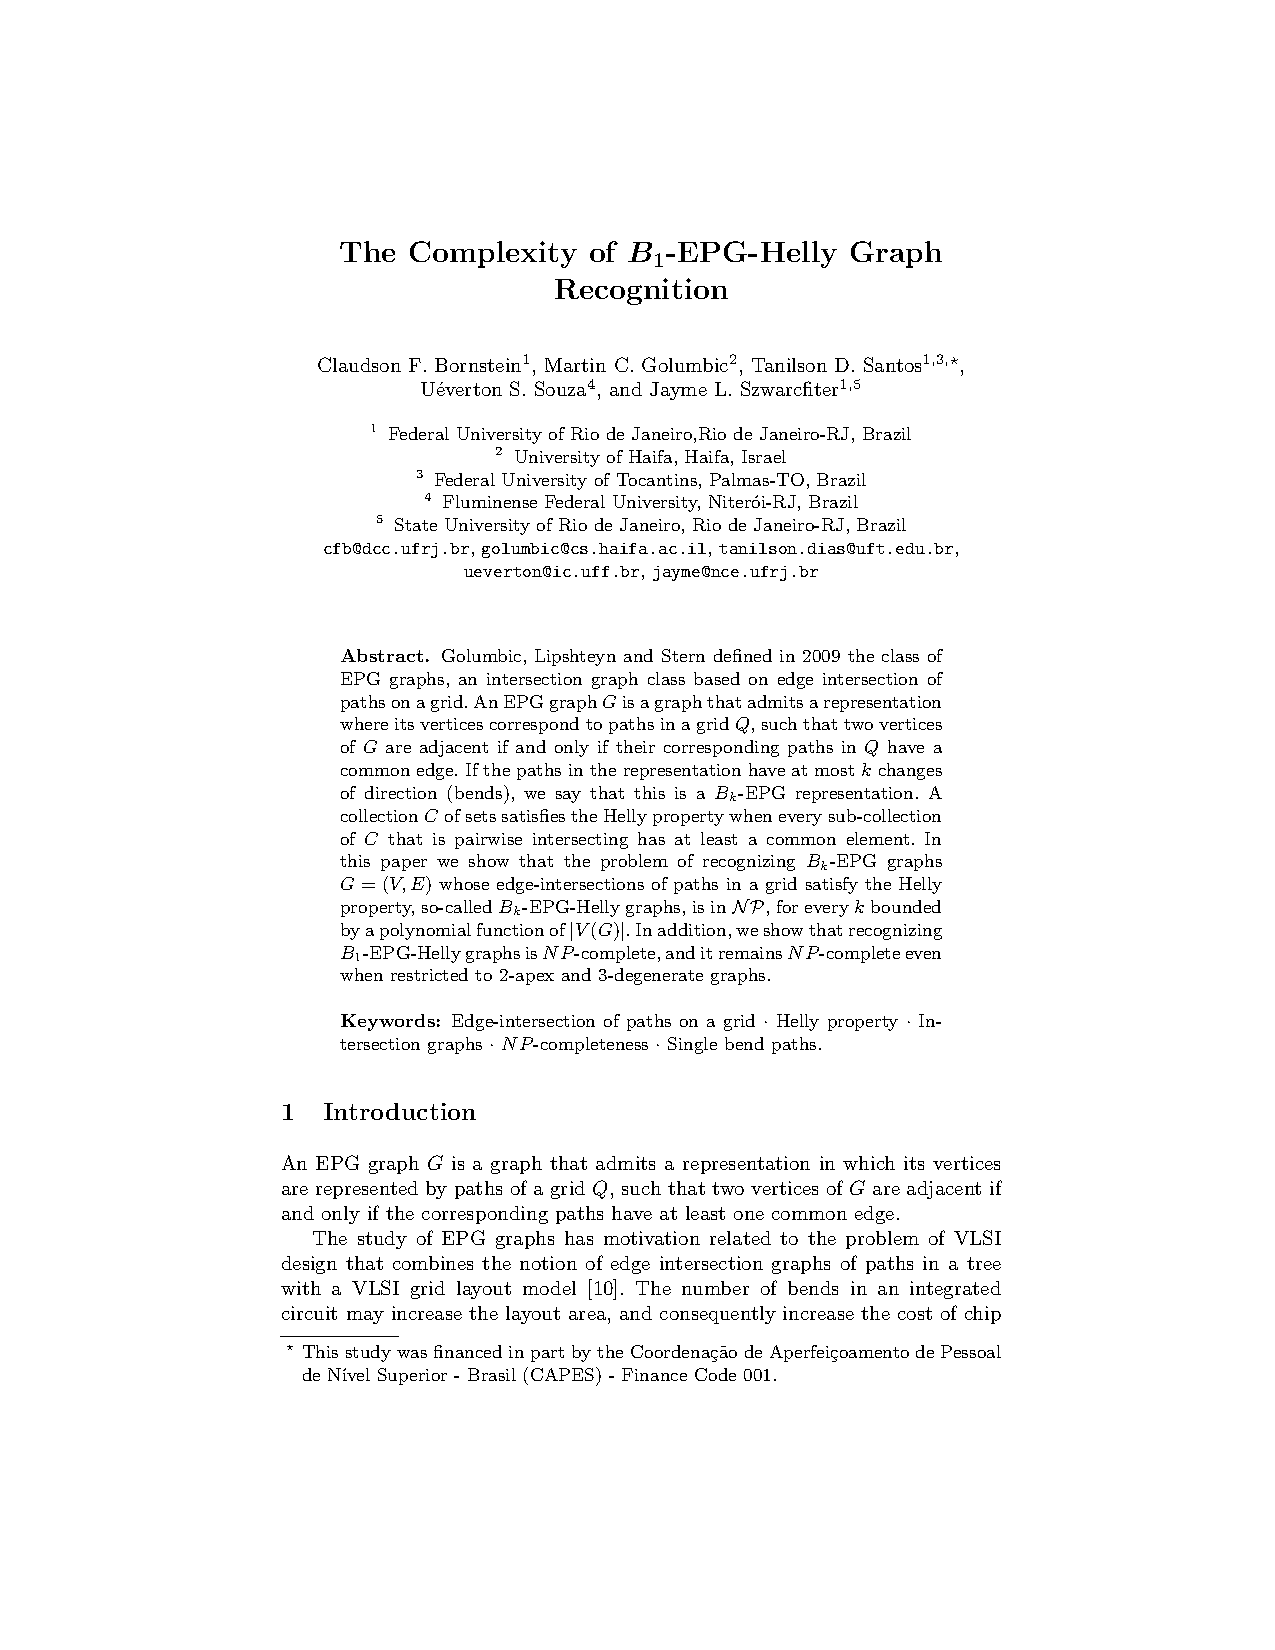
\includepdf[pages=-]{./includes/include-pdf-files/wg2019.pdf}
\label{appendix}
  
  \printindex   % Se não tiver indice remissivo pode remover
\end{document}
